
\section[Generating predictive representations in the manual modality]{Generating predictive representations\\ \hspace{.31in} in the manual modality}
    \setcounter{page}{1} \renewcommand{\thepage}{\arabic{page}} 
    \subsection{Introduction}
            %    
                A plurality of evidence points to the notion that observation and comprehension involve some form of short-term prediction \cite{kutas2011, wilson2005}. Both action and language comprehension are said to rely upon anticipatory predictive representations, also called forward models \cite{PG}. Existing theoretical work on forward modeling derives the majority of its evidence from spoken language and object-oriented action, but a true test of theoretical claims would examine linguistic and nonlinguistic predictions in the same context. Do theoretical claims about predictive representations hold true for both linguistic and nonlinguistic manual information? What about manual language may differentiate findings from existing literature on spoken language? And to what extent are predictive abilities tied to theoretically related motoric abilities? \par
                Experiment 1 of the present work directly compares predictive representations for manual language and similar nonlinguistic body-oriented gestures to address (a) claims about the similarity of linguistic and nonlinguistic predictions and (b) the lack of sign language research on forward modeling. Experiment 2 delves further into an arguably unique attribute of manual languages that supports predictive reorientations, transitional periods, and, in so doing, addresses additional questions about the use of different phonological features in generating predictions. Experiment 3 then examines tasks that were hypothesized to support predictive motoric processing, memory and motor imagery. Finally, Experiment 4 directly compares participant performance across Experiments 1, 2, and 3 to draw conclusions about the nature of predictive representations under various task conditions and under what circumstances memory and motor imagery play a role in the predictive motor representation process. \par
                To appropriately address the motivation for these Experiments, this introductory Chapter will, first, cover the theoretical proposal that has guided the present work. Second, this Chapter will discuss the features of sign language that differentiate investigations with sign language and gesture from existing spoken language research, as well as review sparse existing evidence of predictive processing in sign language. Third, the present chapter will highlight the relationship between theoretical proposals for motoric simulation as a comprehension mechanism and related motoric cognitive abilities, such as memory and imagery.
    \subsection{Action as a Basis for an Integrated Language Model}
            Standard, more modular theories might define language production and comprehension as separate, sequential processes. An individual's mechanism for comprehension would take a physical stimulus, decode it into basic linguistic components, and apply some form of processing to derive each successive linguistic level, in order to generate an amodal semantic representation. After the individual has formulated a desired outgoing message, a separate process for language production could then re-code the message into an utterance. In a modular, sequential processing stream, language is the medium through which abstract thought is communicated, but only via rapid and repeated coding and decoding, to and from language as a substrate.  \par 
            Pickering and Garrod \citeyear<\i{P\&G};>[]{PG}, by contrast, make the case that (a) nonlinguistic action production and action perception are highly intertwined, (b) language is a specialized form of action, and, as a result, (c) language production and comprehension must be similarly intertwined. The specific mechanism said to underlie production and comprehension, in both linguistic and nonlinguistic cases, is predictive motor simulation. According to P\&G, simulation is the means by which individuals plan both linguistic and nonlinguistic acts and self-monitor for errors. And simulation is what gives rise to comprehension, via detailed predictive representations of others. By understanding simulation in the case of action production and comprehension, P\&G formulate their testable proposal for language \i{forward models}. \par
            In brief, a forward model is a comprehensive representation that predicts the next step in an ongoing stimulus. While attending to an interlocutor, an individual would develop a forward model to represent all aspects of the interlocutor's action or language: motor movements, goals, meaning, and possible linguistic features like syntax, morphology, and so forth. A \i{forward model} refers to the entirety of this representation. As it is difficult to assess the entirety of predictive representations experimentally, the present work will often refer to \i{predictive representations} to discuss mental representations constituent to, but not the entirety of, forward modeling processes. Nevertheless, it is important to understand the nature of P\&G’s more comprehensive proposal in order to understand the present work’s contribution to this field.\par
        \subsubsection{Forward Modeling: Action}
            In the simple act of reaching out one's hand to pick up an object, there are many unconscious calculations made to fine-tune the muscles involved. Flexion of the fingers depends on the size of the object, tension of the wrist depends on anticipated weight, and, once the object is grasped, visual and proprioceptive feedback mechanisms allow us to adjust these predictions about ourselves, and about the consequences of our own actions, based on new information. P\&G use Wolpert's motor planning proposals \cite<e.g.,>[]{davidson2005,wolpert1997} to describe an action production system that would generate predictive forward models about the outcome of grabbing a cup, for example. A prediction about picking up a full cup would specify the weight to be expected against the hand. In the event that the cup were empty, such a detailed model would facilitate rapid course-correction in order to avoid throwing the cup into the air. These predictions are possible, in part, because the motor commands responsible for generating the action are, in some form, available to the forward action model. This secondary pathway, the authors suggest, is the means by which the production system self-monitors so readily \cite{davidson2005}. \par
            P\&G argue that forward action models are used not only to predict one's own actions, but also to predict the actions of others. In contrast to the above case, predicting the action of others does not come equipped with a secondary copy of the exact motor command. Instead, an observer must simulate the relevant motor commands for the observed process. A lifetime of associative learning allows perceivers to intuit the appropriate motor commands for a relevant action and covertly simulate the observed act via the observer's unique motor system. Although some adjustments are made based on the features of the perceived actor, there is evidence that the predictive representations generated about others are primarily based on knowledge of oneself, and, therefore, have an \i{egocentric bias} \cite<e.g.,>[]{knoblich2001}. That is, the default prediction of an observed action will be based on a detailed understanding of one's own body, either facilitating predictions when the observed individual and the observer would somehow conduct the action similarly, or giving rise to errors when the two differ. \par
            In the context of P\&G's model, egocentric covert imitation gives rise to a detailed forward model, which is sent forward to a comparator node. This node provides feedback in the event that there is a mismatch between the forward model and observed action (either for oneself of another). Egocentric biases are borne out of a mismatch between a generated prediction and observed action. They therefore require (a) sufficiently detailed predictions and (b) a stimulus, internal or external, that does not align with the prediction. \par
            Evidence that these motoric simulations are active can be found in magnetoencephalography (MEG) data pointing to primary motor area activation in pianists listening to piano music \cite{haueisen2001}. Evidence that these simulations are based on the self also stems from studies that show better predictions when watching one's own actions compared to those of another \cite{knoblich2001}. For example, Knoblich and Flach (2001) showed participants videos of themselves and another participant throwing darts. Participants were asked to predict where the dart would land. In one condition, only the arm was shown to limit the use of gaze and body posture in generating predictions. Participants were marginally more accurate when predicting videos of themselves compared to those of another person. In the framework described above, participants were using their action execution system as a means of generating predictions. Individual idiosyncrasies in dart throwing lead to an egocentric bias in forward models. \par
        \subsubsection{Forward Modeling: Language}
            The focus of the present work, however, is the intersection of action and sign language in predictive modeling. P\&G use the action framework described above to discuss their proposal for self-monitoring during spoken language production, and motor simulation during speech comprehension. Production and comprehension are so highly intertwined, P\&G claim, that when a language production command is issued to articulators, this command is rapidly simulated by a forward model for each linguistic level: phonology, morphology, syntax, etc. Just as in action, the outcome of actualized production is compared against sensorimotor feedback to rapidly monitor for errors. Just as one adjusts muscle tension to compensate for unexpected weight in the cup example, comparing sensorimotor feedback of a phoneme to the predicted utterance allows speakers to make fine adjustments to articulators. P\&G highlight evidence that individuals both modify speech production and show differential MEG response within 100 ms of receiving altered sensory feedback (e.g., pitch shifted feedback) \cite{tian2010,tourville2008}. \par
            During language comprehension, P\&G propose that the same forward model is at play via \i{covert imitation}. By subvocally reproducing the language input, a comprehender derives a language production command, which, in turn, generates a forward language model. For evidence of covert articulation, P\&G point to shared areas of activation for both hearing and producing specific phonemes \cite{pulvermuller2006,pulvermuller2010}. For evidence that this articulation feeds predictive models, P\&G discuss a number of studies. \citeA{mottonen2009}, for example, found impaired phonemic categorical perception when participants' speech-motor areas were disrupted via transcranial magnetic stimulation. By disrupting covert imitation in motor speech areas of these participants, researchers impaired the predictive model, and therefore language comprehension.\par
            By generating a covert imitation production command and a subsequent predictive model, comprehenders can compare predictions with additional language input. Rather than preventing errors in a self-monitoring process, such \i{other-monitoring} facilitates well-coordinated conversations. Because this predictive model is based on the comprehender's own experience with language, P\&G suggest that there will be some degree of egocentric bias in the prediction; one's forward language models should be primarily based on one's own experience producing the language, inclusive of articulatory idiosyncrasies, word choice habits, etc. P\&G acknowledge that some aspect of the system must consider context, however. The context module of P\&G's model allows comprehenders to incorporate producer-specific information into forward models. Exactly what kinds of information can be incorporated is underspecified, but, for the purposes of the present discussion, egocentric biases will serve as a tool for experimentally probing the nature of forward language models in sign language users.\par
            \label{sec:intro_shad_spoken} Much of the validation for proposals of egocentrism in forward language models comes from shadowing paradigms. This experimental setup, developed by \citeA{christo1960}, asks participants to shadow, or closely repeat, incoming information. In spoken language, this can take the form of a participant repeating incoming auditory input as soon as possible after hearing it. By measuring time delays between the input and the shadow (i.e., lag time), experimenters can directly measure how efficiently participants can anticipate input. Different studies have assessed how predictions are influenced by syntactic constraints \cite{marslen1985}, regular phonemic changes \cite{brouwer2010,fowler2003}, allophonic variation \cite{honorof2011}, etc. 
            %\citeA{miller2013} examined how speakers slowly shift from egocentric responses to incorporating model-specific information in shadowing responses.
            \citeA{nye2003} demonstrated greater alignment to a shadowing stimulus that conformed to participants' native language phonotactics. For full review of shadowing literature in the context of the P\&G (2013) framework, see \citeA{gambi2013}. \par
        \subsubsection{Summary}
            P\&G derive inspiration from the forward action modeling literature to put forth their own proposal for forward language modeling. In both action and language, a motoric simulation of an act facilitates predictions about the outcome and facilitates rapid accommodate of unexpected outcomes. This process is said to apply to both predictions generated for oneself, as well as those persistently passively generated for others in the process of action and language comprehension. Because the driving mechanism behind forward models is motoric simulation, errors are prone to egocentric bias. When predictions are flawed, errors patterns exhibit characteristics of individual generating the forward model, rather than the observed stimulus. This bias has been used in experimental investigations of spoken language \cite<see>[]{gambi2013}, and is again the target of investigation for Experiment 1, as presented in Chapter 2 of the present work. \par
            P\&G make the case that action and language predictive representations differ in degree of complexity but not qualitative kind. Prior evidence has been limited insofar as comparisons must be made across experimental contexts: spoken language and action cannot be compared with the exact same methodology and, instead of performing direct comparisons on a dataset, P\&G point to common patterns such as egocentric bias to make the case for motor stimulation. Experiment 1 (a) extends existing language forward modeling results to sign language and (b) provides a direct comparison between action and language forward models, for individuals both familiar an unfamiliar with the language in question, American Sign Language. There are reasons to believe, however, that a change in language modality may be associated with a unique relationship between language and action predictions. The following sections provide a brief overview of sign language linguistics as well as existing evidence of forward modeling-like predictions in the manual modality. 
    \subsection{The Overlap between Action and Language in Sign}
        \subsubsection{Why Sign Language?}
            When considering language as action, sign language offers the closer comparison with actions in order to validate P\&G's claims simply because sign and actions (of the sort described by P\&G) employ the same articulators and are, therefore, more likely to employ similar predictive processing mechanisms. In the case of spoken language, the majority of vocal articulators are not available in the same modality as the resulting language output: most articulators are hidden from sight and perceptual contrasts of spoken languages are auditory. To derive the action command (or the motoric specifics) of a speech sound, a comprehender must rely on associations between auditory information and vocal actions, rather than relying on direct visual evidence of muscle movements, as in the case of sign. The vocal articulators are also relatively specialized in their use. \par
            Sign language, by contrast, offers full visual access to the linguistic articulators, simplifying P\&G's proposed associative learning for generating motor commands in covert imitation. And, the overlapping nature of articulator use across both action and sign language would theoretically lead to an even more intertwined relationship than has already been observed. Offering full visual access to articulators, however, forces the language stream to be persistent. The spoken language stream can be temporarily ceased when transitioning between words by discontinuing vocalizations, but the visual nature of sign language forces transitions between words to be visible.  The present work will discuss the fluid sign stream in terms of segments: signs and transitional periods \cite<see>[for review]{jantunen2013}. Sign language users may differentially employ transitional information in generating predictions about nonlinguistic actions. Transitional movements may not be regulated by phonological principles, and sign language users may be in a position to generalize their understanding of transitions beyond linguistic contexts. \par
            While a more extensive investigation of sign language forward models would cover these predictive representations in their entirety, as they are informed by syntactic and semantic structure, the following Chapters deal strictly with phonological information in predictive representations to facilitate later comparisons across signers and nonsigners. As such, the following section will provide an overview of sign phonology to facilitate specifics in later chapters, covering the utility of transitional information in generating predictive representations as well as the limited existing evidence for egocentric bias in single-sign processing. \par
        \subsubsection{Sign Phonology and Transitions} 
            \label{sec:intro_phono}
                The phonological structure of sign language is generally characterized in terms of components or parameters of sign form \cite<e.g.,>[]{sandler2006}. These separate parameters are, to some extent, parallel to the separation between consonants and vowels in spoken languages \cite{orfanidou2009}. Among these parameters, those chiefly relevant to discussions of predictive representations include handshape, location and movement. \par
            \subsubsubsection{Handshape}
                Hand configuration, or handshape, is characterized by positioning of the fingers (and thumb) of the hands. Sign languages differ in the number and specifics of the handshapes of their permissible inventory. Early ASL sign researchers such as Stokoe \citeyear<>[reprint]{stokoe2005} listed approximately twenty handshapes for ASL, but linguists have since identified more contrastive handshapes (approx. 40) and provided more detailed theories regarding the role of features in generative grammar \cite{brentari1998}. One way to discuss this set is to use the linguistic notion of markedness to characterize handshape complexity. \citeA{brentari1998}, p.~118, in Stokoe notion \cite<>[reprint]{stokoe2005}, defines the set of unmarked (i.e., less complex) handshapes as B, A, S, C, O, 1 and 5. These are the handshapes with either only one or all fingers selected  \cite<i.e., actively engaged; see>[]{mandel1981,brentari1998}. In the context of Brentari’s model, selected fingers must be specified with additional flexion and spread information (i.e., how curled is the finger and how far apart are fingers from each other). Intuitively, the more details to be represented in specifying a predictive representation for handshape, the greater cognitive demand required by such a prediction\footnote{For review of variation in handshape complexity in natural signing, see \citeA{eccarius2007}.}. While handshape is routinely paired with additional phonological information to give rise to a well-formed sign, but \i{fingerspelling} serves as a case where detailed representations are generated primarily based on sequential presentations of complex handshapes. Fingerspelling has been described as a system for presenting orthography \cite{geer2017}\footnote{For a more in-depth discussion of the role of fingerspelling in ASL, as well as the relationship between ASL fingerspelling and English, see \citeA{brentari2001}.}.  In ASL, signers use signs to rapidly spell out English words, possibly because no such sign exists (e.g., brand names, novel technical terms, etc.). While some letters employ short movements or palm orientation changes, fingerspelled letters in ASL are primarily unique handshapes. Researchers refer to the presented letter as a \i{hold}, \cite{schwarz2000, wilcox1992}. Commonly fingerspelled words undergo a lexicalization process that may reduce the articulation of certain holds or skip others altogether according to principles of lexicalization, or \i{naturalization} \cite{cormier2008}. While the end result of this process is a lexicalized sign, in the sense that it may not be understood as having fingerspelled constituents, various forms along the naturalization process would task signers with comprehending intermediate handshapes that do not necessarily fit within the defined inventory. \par 
                \citeA{geer2017} reviews evidence that deaf signers attend more to the overall shape of the word. \citeA{akamastu1985} describes children attempting to fingerspell whole words, rather than individual letters, and reports an anecdote of a child who only later realized a gestalt sign she produced was comprised of fingerspelled components \cite<as cited in>[]{maxwell1988}. \citeA{schwarz2000} investigated signer perception of fingerspelling videos without hold segments and found that signers can derive some information from transitional periods alone, such as overall height \cite<as cited by>[]{geer2017}. Novices, on the other hand, demonstrated greatest accuracy from isolated hold segments in comparison to natural fingerspelling or transition-only conditions \cite{geer2014}. To further investigate how sign novices perceive fingerspelling and acquire comprehension techniques, \citeA{geer2017} provided participants with either (a) standard classroom exercises to reinforce the ASL alphabet, or (b) explicit training in the contrast between transitions and hold fingerspelling segments, as well phonetic variation (i.e., how a letter may look noncanonical in context). Only novices with explicit training showed improvement in fingerspelling comprehension. While novices can be trained in attending to transitional information \cite{geer2017},  the transitional periods during fingerspelling are certainly more informative to experienced signers who are familiar with phonological naturalization processes and focus on the gestalt perception, rather than individual letters \cite{wilcox1992}. \par
            \subsubsubsection{Location}
                In fluent signing, handshapes are simultaneously paired with location and movement information. Locations are typically described as either (a) positions relative to the body (e.g., head, chin, chest) or (b) occurring in neutral space, the area in front of the signer. \citeA{mauk2003} documented evidence that sign location height during sign production is influenced both by the height of neighboring signs, as well as the speed of production. Signs presented in neutral space, as well as high frequency signs, were the most susceptible to co-articulatory changes in height \cite{mauk2003, mauk2008}. Research on the perceptibility of such a cue in generating predictions is limited to one case that explicitly informed participants of co-articulation effects. \par
                Specifically \citeA{grosvald2012} showed participants sentences of the form I WANT (X), I WANT FIND (X) and I WANT GO FIND (X), where (a) X was a sign with either high or low elevation and (b), for experimental items, the video ended before X. Participants in both signer and nonsigner groups were able to guess the height of X using co-articulation height information present on WANT, and sign language exposure had no effect on performance. This finding should be interpreted, however, knowing that task instructions explicitly highlighted the possibility of long-distance co-articulation in linguistic stimuli. Additionally, the practice phase for this task began with full I WANT (X) videos that explicitly showed the target item, and slowly transitioned to the experimental items lacking the target X. The nature of these instructions and practice likely facilitated awareness of height co-articulation for both groups. It remains to be seen if nonsigners would perform similarly without explicit instruction, and whether or not speed of movement, as described by \citeA{mauk2003}, prior to X is a sufficient source of information to make a similar judgment. Experiment 2 of the present work specifically focuses on the utility of transitional movement in sign identification. \par
            \subsubsubsection{Movement}
                Broadly speaking, movement in sign phonology can refer to (a) a path the hand(s) take from one location to the next (e.g., moving from the chin to the chest), (b) a change in handshape (e.g., changing from a fist to an open handshape), (c) a change in hand orientation, or (d) a combination these movement types \cite{sandler2006}. The first kind of movement, path, is lexically specified and can take many forms: straight, arcing, circular, etc. Sequential syllables in ASL can be distinguished based on these sequential movements \cite{corina1993}. These movements within sign production have been shown to have less velocity and more acceleration than the movements that must occur between lexical items \cite{jantunen2013}. In other words, lexical movement is produced more slowly than transitions, but takes less time getting up to speed. \citeA{jantunen2013} describes signs as maximizing the amount of time moving at the appropriate communication rate, while transitions are far more variable. Because transition movements do not have specified lexical representations, it may be the case that they are purely regulated by the same efficiency and biomechanical principles that would govern nonlinguistic action. Section \ref{sec:intro_trans_predict} will review existing evidence that signers make use of transitional information during sign language comprehension. In light of the potential similarities between linguistic and nonlinguistic transitions, this Chapter will provide a basis for predicting knowledge transfer from language comprehension to action perception in sign language users, in advance of the empirical investigation to this effect in Chapter \ref{ch:trans}. \par
            \subsubsubsection{Articulator engagement and symmetry}
                \label{sec:intro_sym}
                The discussion of handshape above highlights how providing additional information articulator complexity handshape serves as an additional cognitive demand in generating a mental representation. Specifying an entire additional articulator might logically also be more cognitively demanding, but this notion does not bear out in sign language processing literature. The fact that sign language makes of two large, independent articulators does not have a clear spoken language parallel \cite{shield2018} and makes for several interesting relationships to predictive representations more broadly. First, the hand an individual uses when producing one-handed signs is tied to hand dominance. Studies presented in Section \ref{sec:intro_sim_sign} exploit this fact to look for evidence of egocentric bias, and therefore motor simulation in sign perception. Second, and the focus of the present section, executing a one-handed sign is counter-intuitively more difficult due to a natural tendency for motor activation to be mirrored across the two hands. \par
                \citeA{battison1978} is famous among the sign language research community for outlining the \i{symmetry} and \i{dominance} constraints on sign language production \cite<as cited by>[]{eccarius2007}. The former states that, if the hands move independently in sign production, they will be specified with the same handshape, location and movement. The latter states that, if the hands are specified with different handshapes, the non-dominant hand will be passive in movement and is limited to unmarked handshapes. Battison (1978) labels two-handed asymmetrical signs as Type 3, the most complex. Two-handed signs with shared handshape, but passive and active movements, are Type 2. Type 1 signs are symmetrical two-handed signs and, finally Type 0 signs are one-handed. By implication in Battison’s (1978) system, one-handed signs are the least complex, but evidence from natural production data and neuroimaging evidence indicates that one-handed signs may be as complex as Type 2 or 3 in terms of cognitive demand. \par
                \citeA{meier2006} summarized evidence of production errors during sign language acquisition. In particular \citeA{meier2006} documented cases of children exhibiting sympathetic articulation during asymmetric productions (i.e., either Type 0, 2 or 3).  In cases reported by \citeA{meier2006}, the non-dominant hand, in early childhood productions, had a tendency to mirror the dominant hand in either movement, location or both. \citeA{meier2006} even suggested that children may be avoiding Types 2 and 3 signs as a result of their difficulty. These sympathetic productions might be described as a spreading of activation from dominant to non-dominant hand. A lesser incidence of these errors in adult signers would, then, be indicative of an ability to suppress similar activation. \par
                \citeA{hickok1996} documented evidence of an adult aphasic signer who exhibited similar sympathy in asymmetric productions (movement and handshape) for one-handed signs. Damage to left anterior frontal areas (Broadmann’s 44/45) may have resulted in reduced ability to suppress non-dominant hand activity. In a related neuroimaging study with native neuro-typical signers, \citeA{emm2016} found greater activation associated with one-handed sign production in adjacent the left inferior frontal gyrus, an area associated with motor suppression \cite{swick2008}. \citeA{emm2016} discussed this finding as evidence that the motor command is spread across the two hemispheres when engaging in a two-handed production, but the same activation could be interpreted as non-dominant hand suppression during the production of a one-handed sign. \par
                \citeA{emm2016} contextualized their finding in relation to similar studies regarding the increased premotor activity associated with nonlinguistic one-handed tasks \cite{knocke2004, post2007}. Additional neuroimaging evidence examined one-handed tapping with both the left- and right-hand among right-handed individuals. \citeA{aramaki2006} presented evidence that non-dominant hand tapping does not impact the primary motor cortex for the dominant hand, but dominant hand directly suppresses non-dominant motor cortex activity. In other words, interhemispheric motor suppression was unidirectional, from dominant to non-dominant sides. Vines and colleagues directly investigated intra-hemispheric suppression, as well as motor suppression asymmetries, via transcranial direct current stimulation and reinforce the notion that, in the context of low-level motor activation, one-handed productions result in non-dominant hand suppression \cite{vine2006,vine2008a,vine2008b}. It is difficult to tie this kind of minimal movement, tapping, to much more comprehensive motor planning tasks, but the evidence for non-dominant hand suppression exists on the level of interhemispheric neuronal connections. \par
            \subsubsubsection{Phonology summary}
                In sum, \citeA{battison1978} implies that one-handed signs should be less complex than two-handed signs. Intuitively, one would assume that an additional articulator (i.e., the non-dominant hand) would render a production (or simulation thereof) more complex. Instead, the default mode of manual productions may be to send symmetrical signals to both hands \cite{meier2006, hickok1996}. In the case of a one-handed sign, one signal would be sent to the dominant hand, and a suppressive signal would be sent to the non-dominant hand \cite<e.g.,>[]{aramaki2006}. Experiments 2 and 3 will rely on this proposal for interpreting differences in responses to one- versus two-handed stimuli.
        \subsubsection{Transitional Information in Sign Predictions}
            \label{sec:intro_trans_predict}
            Following the work by \citeA{jantunen2013}, the transitional period of the fluid sign stream was defined to begin as soon as the dominant hand diverts from the movement specified by a given sign. This period ends immediately prior to the specified movement for the subsequent item. With this definition in mind, a number of sign language comprehension studies can be understood as providing evidence that comprehension incorporates information prior to the onset of the target sign, both in sentence and response-to-target contexts. Evidence from electrophysiological research, in particular, highlights the degree to which signers make use of transitional information in ordinary sentence comprehension\par
            In an event-related potential (ERP) study, Hosemann and colleagues \citeyear{hosemann2013} examined brainwave patterns, namely the N400 component, in response to German Sign Language (DGS) sentences, with either semantically predictable or unpredictable endings. For example, \i{a rabbit jumps across a path} is much more predictable than \i{a crocodile jumps across some meat}. Per DGS syntax, JUMP is the last sign in each case, but, if the established nouns are CROCODILE and MEAT, EAT is the expected verb and JUMP is anomalous. 
            Ordinarily, the N400 is observed 400 ms after semantically anomalous information. In the case of \citeA{hosemann2013}, N400 effects were seen from 0 to 350 ms after the onset of the anomalous sign. In other words, information in the transition to the sign JUMP shaped predictions before the sign was fully realized. The information required to recognize an anomalous sign may occur up to 400 ms before the onset of the sign itself. Signers are therefore using preparatory transition movements for sign recognition.\par
            Arendsen, van Doorn and de Ridder \citeyear{arendsen2007} provide some additional evidence for the informative nature of transitional movement in a study that examined sign recognition reaction times for both signers and nonsigners. More specifically, this study presented participants with mixed sequences of signs in Sign Language of the Netherlands (NGT) and distinct \i{grooming gestures} (e.g., scratching the nose, running hands through hair). The signs and gestures were produced in fluid strings, including transitional movement either from a rest position (hands on a table) or from the preceding item. Participants were instructed to press a key whenever they identified a sign. In P\&G's terminology, \citeA{arendsen2007} asked participants to construct forward models of manual output and to respond as soon as they had sufficient evidence to identify a sign. Both deaf and hearing signers could draw on their knowledge of NGT, while the non-signers made this judgment purely based on the manual form. \par
            On average, all participants identified the sign 200 ms after sign onset, but signers were 90-150 ms faster than nonsigners at identifying signs, which is indicative of language experience giving rise to richer or more efficient predictive models. Importantly, across all participants, there was a negative correlation between the duration of transition movement and response time after stroke onset. In other words, the longer the sign model took to transition, the quicker participants identified a given item as a sign. In the case of the signers, transitional movements likely informed the linguistic process of sign identification. For the nonsigners, the explanation for the correlation is less clear. Are nonsigners sensitive to linguistic elements of transitional movements for categorization? What components of this manual stream are useful predictive evidence for either group? Experiment 2 will address these questions. Experiment 1, however, covers the more basic question of whether or not signers employ forward models in the way P\&G have described.
        \subsubsection{Selective motor simulation in sign processing}
            \label{sec:intro_sim_sign}
            Existing evidence regarding the use of motoric simulation to facilitate sign language comprehension can be found in single sign comprehension tasks. Here, hand dominance is used to look for egocentric bias in lexical decision and match/mismatch tasks. While such evidence is present, it is limited to specific cases and, therefore, calls for a more direct examination of forward models of the sort presented in Chapter \ref{ch:shad}. \par
            Corina and Gutierrez \citeyear{corina2016} presented right-handed signers with a series of signs and pseudosigns (phonotactically permissible, but non-existing signs), which were either presented as filmed with a right-handed model or mirror reversed to give the impression of a left-handed model. Participants were asked to make a lexical decision: either respond yes or no to identify true signs and reject pseudosigns. \citeA{corina2016} base predictions on a motor-simulation theory of language comprehension, and contrast participant performance on handedness-aligned versus misaligned stimuli. In accordance with predictions, participants responded more quickly to handedness-aligned items. Interestingly, participants were faster to reject misaligned pseudosigns, perhaps suggesting a task-specific effect whereby more efficient motor stimulations render pseudosigns harder to reject. \citeA{corina2016} note, however, that these effects are limited to non-native signers, suggesting that motor simulation may not be observable in a lexical decision task for native signers. Native signers are already so efficient at sign recognition, the authors argue, that the handedness incongruence cannot impact performance. While the notion of a ceiling effect for native signers in \citeA{corina2016} remains valid, more recent evidence revisits conclusions regarding motor simulation by testing both left- and right-handed subjects. \par
            Watkins and Thompon \citeyear{watkins2017} conducted a similar sign perception task focused on handedness. Native and non-native signers saw pictures followed by individual signs, presented as either a left- or right-handed model. Participants simply indicated whether or not a given sign matched the preceding picture. By recruiting both left- and right-handed participants, authors were able to parse the effect of frequency from handedness-alignment effects. As the majority of the population is right-handed, right-handed productions are far more common. Overall, \citeA{watkins2017} report a main effect of model handedness, whereby response times were overall faster for right-handed productions, regardless of participant handedness. In this match-mismatch case, frequency of exposure seems to play a major role in response time, for both right- and left-handed signers. \par
            \citeA{sharma2014} found a similar familiarity effect when asking both left- and right-handed signers to sign with their non-dominant hand; left-handed signers produced fewer errors than right-handed signers \cite<as cited by>[]{shield2018}. Sharma’s (2014) left-handed participants may have, by visual familiarity alone, had stronger motor representations for right-handed productions than their right-handed counterparts had for left-handed productions. By extension of this notion of visual familiarity, it may be the case that responses to more familiar stimuli, like one’s friend versus a stranger, may be similarly expedited. Experiment 1 of the present work explores this idea further. \par
            There was one exception to the frequency of exposure trend in \citeA{watkins2017}: left handed signers showed congruency effects (faster response times to left-handed productions) only for two-handed asymmetrical signs. These phonologically complex signs involve two different handshapes and \citeA{watkins2017} propose that motoric simulation is a modulating factor in, rather than a primary mechanism for, sign comprehension. \citeA{hickok2011} provide a review and critique of spoken language forward modeling literature to similar effect: motoric simulation may only be a supportive mechanism under difficult or uncertain conditions. The same logic for relative phonological complexity could be applied to different groups, native vs. non-native, with more or less ease in completing the task \cite{corina2016}. \par
            It is difficult to judge a priori whether or not a task would be sufficiently difficult to elicit the theorized motor simulation. \citeA{hickok2011} highlight stimulus ambiguity and temporal constraints as playing major roles in this regard; if the stimulus is sufficiently noisy or a response must be generated quickly, motor simulation may support existing processes. It may be the case that ordinary sign comprehension in the context of the experiments presented above \cite{watkins2017, corina2016} do not sufficiently tax comprehension mechanisms in order to activate motor simulation. Only in the case of two-handed asymmetrical signs is the visual information sufficiently complex to require additional support from motor simulation. Experiments 1 and 2 of the present work employed more time-sensitive tasks to elicit motor simulation, either by directly engaging the participants’ expressive motor system in Shadowing, or requiring persistent stimulus monitoring in a response-to-target task. 
    \subsection{Facilitating predictive representations}
            The notion that motor stimulation may be one component of full predictive representations gives rise to questions regarding what other cognitive abilities may play a role in predictive language processing. Huettig and Janse \citeyear{huettig2016} describes visuo-spatial memory as facilitating eye-tracking predictions. \citeA{donoff2018} presents a novel task examining motor imagery that, while not predictive, would likely share resources with a motoric simulation mechanism. \par
            More specifically, \citeA{huettig2016} presented participants with many variations on the following sentence in Dutch: “look at \i{the} displayed X,” where X could be a number of different nouns that took either the common or neuter gender of the article \i{the}. At the same time, participants were visually presented with four pictures of objects, and an eyetracker was used to monitor gaze. For any given trial, the target picture was the only item presented with the relevant gender. Considering this task alone, \citeA{huettig2016} examined whether or not participants could generate predictions based on article gender and direct gaze to the target item. On average, participants demonstrated such an ability, with proportion gaze to target significantly above chance 2000ms after article onset. \par
            This eyetracking task, however, was paired with measures of processing speed \cite<digit-symbol substitution;>[]{wechsler2014}, as well as both auditory \cite<non-word repetition;>[]{wechsler2014} and spatial memory \cite<Corsi block test;>[]{corsi1972}. The authors then examined the relationship between amalgam measures for both processing speed and working memory to demonstrate a significant relationship between each measure and a given participants’ proportion gaze to the target. \citeA{huettig2016} make the case that an individuals’ ability to retain the set of visually presented objects in working memory is related to an ability to make linguistic predictions in this task. Experiment 4 of the present work will further explore this link with a memory task more targeted to the manual modality. \par 
    \subsection{Summary}
        %
            P\&G discuss both action perception and spoken language comprehension systems as being driven by the same motoric simulation processes that gives rise to detailed predictive representations, also called forward models. The parallel between action and language is proposed, however, on the basis of seeing similar patterns of results, including egocentric bias, across different experimental designs \cite{PG}. There is no reason to believe these results would not extend to sign language, and even some evidence to suggest the relationship between action and language would be stronger across a shared modality. \par
            Sign may differ from speech, however, insofar as the sign stream is comprised of clearly delineated purposeful versus transitional periods that are directly observable \cite{jantunen2013}. Signers may, as a result of experience generating predictions based on linguistic transitional periods, generalize to nonlinguistic contexts. \citeA{hosemann2013} and \citeA{arendsen2007} demonstrate that the immediacy of signer predictive representations for language, but evidence that signers employ motor simulation is mixed \cite{corina2016,watkins2017} and any future studies on motor simulation in sign perception will need to carefully select a task that is sufficiently difficult to solicit such processing \cite{hickok2011}.  \par
    \subsection{The present work}
        %
            The following series of experiments aimed to, first, provide evidence for the use of motoric predictive representations in the manual modality, by demonstrating a key feature of the \citeA{PG} model, egocentric bias. Part of this exploration in Experiment 1 entailed examining (a) how sign language experience impacts both linguistic and nonlinguistic predictive representations, pseudosign and non-linguistic grooming gesture and (b) the role of stimulus complexity in manual predictive representations, via one- and two-handed items. This was accomplished via a Shadowing task that directly asked participants to act out their predictive representations for various stimulus types, grooming gesture versus pseudosign, and stimulus models, themselves, friends and an unknown stranger. Do participants exhibit egocentric biases during time-sensitive manual Shadowing? Is sign language experience associated with any benefits to linguistic and/or nonlinguistic shadowing abilities? Does sign language experience facilitate predictions for particularly difficult stimuli? \par
            Second, Experiment 2 investigated the degree to which forward models rely on transitional information for generating predictions, as well as how sign language users may differentially rely on handshape or movement information in linguistic and nonlinguistic contexts. Experiment 2 employs the same one- versus two-handed complexity contrast as Experiment 1. The task, in this case, required participants to attend to a video and press a button in response to a target item. Stimuli in Experiment 2 are the same as a subset of those presented in Experiment 1, but feature either selective handshape blurring or still frames during transitional information. Manipulating the availability of different kinds of information, handshape and movement, during transitional periods, and testing both signers and nonsigners, allows Experiment 2 to address several questions: does sign language experience promote attention to specific phonological features of transitional periods? And, are differences between groups limited to linguistic contexts? \par
            Third, Experiments 3 and 4 focused on related abilities, including motor memory and motor imagery. This discussion includes both (a) the role of sign language experience in supporting these respective abilities and (b) the role each of these abilities play in facilitating forward models. Experiment 4 also includes an examination of the relationship between Shadowing and the Transitions response-to-target task, as presented in Experiments 1 and 2. \par
            Overall, these experiments aim to (a) gage the role of sign language experience in language and action forward models, (b) measure how sign language users differentially utilize transitional information in forward modeling, and (c) examine sign language users’ forward modeling abilities in relationship to associated tasks (i.e., motor memory and movement imagery). These goals help shape our understanding of language comprehension by investigating predictive motor representations. \par
            % \indent Experiment 1: Shadowing in the manual modality\\
            % \indent Experiment 2: Transitional motion in manual predictions \\
            % \indent Experiment 3: In support of forward models, simulation and memory \\
            % \indent Experiment 4: The relationship between prediction ability, motor memory, and motor \\ \indent \phantom{Experiment 4:} memory \par
        
\section{Experiment 1: Shadowing in the manual modality}  
    \label{ch:shad}
    \subsection{Introduction} 
        %%
            Pickering and Garrod’s (2013) proposal on the nature of forward models relies heavily on covert imitation being used to generate predictions about both action and language. Previous evidence has pointed to familiarity with a stimulus having an impact on predictive abilities \cite{nye2003, watkins2017}. The present Experiment seeks measure the immediacy or strength of forward models across both action and language for both those familiar and those unfamiliar with the language.  This measurement was accomplished by making the covert imitations integral to Pickering and Garrod’s theory observable: making covert imitations overt. Shadowing, as a methodology, does just that: participants are asked to imitate a stimulus as closely in time as possible, and must rely on predictive processing to do so with minimal gap between stimulus and response \cite{marslen1985}. Participants act as a shadow for a stimulus, following along with every movement or syllable. While many studies have employed this methodology over the years \cite<e.g.,>[]{christo1960, marslen1973, scarbel2018}, the majority of this research has focused on spoken language. Here, shadowing was used as a tool for examining both gesture and sign language processing. As participants watched a video, they copied the stimulus with as much accuracy and as little delay as possible. A precise measurement of the delay between an action in a stimulus string and a participants’ shadowed action, the lag time, serves as a dependent measure for participants’ ability to predict an incoming stimulus. The functional purpose of forward modeling is language comprehension, and Pickering and Garrod’s (2013) theorized mechanism for forward modeling is covert imitation. In the present Experiment, covert imitation is approximated by the immediate predictions measured as participants overtly imitate, or shadow, various stimuli. \par
            Although forward language models exist to facilitate predictions on many linguistic levels, including syntax and semantics, the present Chapter focuses on the phonological level to facilitate comparisons across signer and nonsigner language groups. Isolating phonology, in absence of semantics, means focusing on nonwords. Many spoken language studies have asked participants to shadow similar verbal nonsense syllables to examine phonological predictions \cite<e.g.,>[]{honorof2011, miller2013}. The present study employed the manual equivalent of nonwords, \i{pseudosigns} to uniquely focus on how signers’ phonological knowledge may facilitate predictions in absence of semantic or syntactic information. Nonsigers provide a control group for whom the phonological regularities of pseudosign should not impact predictive representations. The closest comparable nonlinguistic actions are grooming gestures (e.g., scratching one’s nose, adjusting one’s hair), as they make use of the same articulators and body-contact while being unguided by any phonological principles. Life-long sign language experience was hypothesized to build stronger internal representations for ASL phonology, as well as develop greater ability to generate predictions based on transitional information, here proposed to be common to both pseudosign and grooming gestures (for more detail, see Section \ref{sec:intro_phono}. Signers were therefore predicted to show greater shadowing ability for both pseudosigns and grooming gestures compared to nonsigners. \par
            Because forward models depend on covert imitation processes unique to the individual, predictions across action and language domains should be more effective when stimuli more closely resemble the characteristics of the participant themselves \cite{knoblich2001, nye2003, watkins2017}. Such an effect reinforces the motoric basis of forward models. The following Experiment involved filming each participant to examine predictive abilities for oneself compared to a friend, as well as an unknown person. Forward models for oneself are theoretically facilitated by the idiosyncrasies of one’s own motoric system, generating an \i{egocentric bias}. A friend, an individual the participant has seen sign and/or gesture regularly, gives a basis of comparison with which the participant is visually familiar, but does not have motoric knowledge. This \i{visual familiarity} may also facilitate predictive processing. The novel third stimulus model showed the same productions produced by a model unknown to all participants. While the friend serves as a baseline for the motoric facilitation of oneself (egocentric bias), the unknown model serves as a baseline for effects of perceptual memory (visual familiarity). The third model also allows all participants to be compared using the same model, in contrast to the other models, which are participant-specific (oneself and one’s friend).  In accordance with \citeA{PG}, motor simulation was hypothesized to regulate all predictive representations, both linguistic and nonlinguistic, and broad familiarity was hypothesized to further support predictive processing. Therefore, participants were predicted to demonstrate the shortest lag times for themselves, followed by their friend, with the longest lag times for the unknown model.\par 
            Across different models, individual stimuli were designed to also allow for comparisons between how participants predict and execute one- versus two-handed signs and gestures. As described in Section \ref{sec:intro_sym}, evidence from child sign language acquisition \cite{meier2006}, aphasiac patient errors \cite{hickok1996} and neural activation patters \cite{emm2016, aramaki2006, vine2008b} point to the notion that symmetrical productions should be considered the default, with one-handed productions requiring non-dominant hand suppression. Briefly, both children and an aphasic patient have shown difficulty with asymmetrical production, while adult signers are perfectly capable of these motor movements \cite{meier2006,hickok1996} and existing neuroimaging contrasts can be understood as greater suppression activity for one-handed productions \cite{emm2016}. \par
            Additionally, sign language use may rehearse ignoring information about hand dominance \cite{shield2018}. Anecdotally, adult signers report that they do not always attend to whether an interlocutor is right- or left-handed; signers remember what was said, but not the specific articulator (right- vs. left-hand) that was used to say it. Nonsigners, however, appear to attend to such information. Anecdotally speaking, many instructors of athletics courses clear up natural initial confusion about how to follow along by instructing participants to mirror (visually observed action on the left equates to left-sided execution) or reverse athletic action. Nonsigners naturally employ a mirroring strategy in copying sign movements \cite{pier2014, shield2018}, instead of choosing to reverse observed movements or making reversal/mirroring divisions based on hand dominance. \par
            In the present experiment, all right-handed participants shadowed right-handed models producing both one- and two-handed pseudosigns and grooming gesture. Nonsigner participants were, therefore, required to fight natural tendencies toward sympathetic movement \cite{meier2006} and mirroring \cite{pier2014}. Participants were instructed to attend to hand dominance and to use their right hand to shadow the right hand of the model. While difficult, this task was expected to be feasible for nonsigner participants and come naturally to signers.. \par
            \phantomsection\label{par:sym_hyp} It was hypothesized that (a) one-handed motor productions and predictive motor simulations require non-dominant hand suppression, (b) non-dominant hand suppression slows prediction mechanisms due to increased difficulty, and (c) regular production of asymmetrical motor movements in sign language rehearses both non-dominant hand suppression and a natural tendency to mirror imitated models. As a result of (a) and (b), shadowing lag times for one-handed items were predicted to be longer than those for two-handed items. And related to (c) above, sign language experience was expected to modulate the difficulty of one-handed items, leading to a reduced difference between one- and two-handed items for signers. \par
    \subsection{Methods}
        \label{sec:shad_meth}
        \subsubsection{Participants}
            Thirty-nine right-handed participants were recruited from the community in San Diego via fliers, online postings, and word of mouth. Participants were recruited as pairs of friends who spend time together in person regularly. 20 Deaf signers (12 Female, \i{M} age = 37.0, range: 24 to 59, \i{SD} = 10.6), with either early or native sign language exposure (age of acquisition $<$ 6), and 19 sign-na\"ive English speakers (15 Female, \i{M} age = 38.8, range: 19 to 64, \i{SD} = 17.5) participated. Nonsigners had no sign experience or minimal sign knowledge (e.g., a few signs or the fingerspelled alphabet). Group sizes were selected to roughly match the number of data points per condition present in \citeA{mitterer2008}. One pair of nonsigner participants was excluded for great difficulty in imitating stimuli during the filming session, one pair of signer participants failed to return for the second visit, and one nonsigner was excluded for failure to complete the task\footnote{This participant's mean reaction time was an outlier relative to other participants. Rather than shadowing, this participant appears to have held items in memory briefly for one third of trials.}.\par
        \subsubsection{Design}
            Participants saw six conditions in a 3 x 2 design: model (\i{Self} vs. \i{Friend} vs. \i{Other}) by stimulus type (grooming gestures vs. pseudosigns). Self stimuli are videos of the participant producing the stimuli set. The Friend model is the other member of the participant pair, an individual with whom the participant is familiar. The Other model is a hearing signer confederate unknown to all participants.\par
        \subsubsection{Materials}
            Grooming gestures, such as scratching one’s nose, rubbing one’s eye, etc., are nonlinguistic actions to which both signers and nonsigners have regular exposure. Twelve common grooming gestures were used in this experiment. Each involved the dominant hand touching some part of the body, including the non-dominant hand, the nose or elsewhere on the head or face. The initial moment of contact is hereafter discussed as the contact point. In addition to familiarity, grooming gestures were chosen because they employ the same articulators as signs, but are clearly non-linguistic and non-communicative. See Table \ref{tab:stim} for list of grooming gesture.\par

            \begin{table}[h] \centering \begin{threeparttable}
    \caption[Experimental items]{Experimental items for Shadowing, Transitions and Working Memory tasks.} \label{tab:stim}
    \begin{tabular}{ll} \hline
    \multicolumn{1}{c}{Grooming Gestures} & \multicolumn{1}{c}{Pseudosigns}\\ \hline
    1.  Tug ear &1.    BACON, one handed, contact ear lobe \\
    2.  Wipe eye &2.    PERIOD, originating at eye \\
    3.  Scratch face &3.    ISREAL, under eyes \\
    4.  Scratch head &4.    DRUNK, contacts head \\
    5.  Rub nose &5.    GREEN, contacts nose, contra-lateral movement \\
    6.  Scratch nose &6.    BORED, R handshape \\
    7.  Push sleeves &7.    WHATEVER, B handshape \\
    8.  Rub Face &8.    BELT, under eyes \\
    9.  Wipe under eyes &9.    BEAR, on head \\
    10. Stretch arms &10.    LICENSE, 3 handshape \\
    11. Twiddle thumbs &11.    TEXTING, inward movement \\
    12. Fold Arms    &12.    BYCICLE, F handshape, synchronized movement \\ \hline \end{tabular} 
    \begin{tablenotes}
        \small \item \i{Note}.
         For images, see Table \ref{tab:stim_app} of the Appendix.
    \end{tablenotes} 
\end{threeparttable}\end{table}   
 

            The pseudosign stimuli were manual productions designed to match grooming gestures in both place of articulation and symmetricity (number of hands involved), while conforming to the phonotactic and phonological constrains of ASL. Pseudosigns were generated by manipulating one or more parameters of an existing sign to create a possible, but non-existing ASL sign. The full item inventory is also listed above in Table \ref{tab:stim}, including glosses (i.e., English translations) of the phonologically closest existing sign and how it was manipulated for form the pseudosign. For set of picutres representing this full inventory, see Section \ref{sec:stim_app}. The first six items in each stimulus type are one-handed items. The latter six are two-handed items. \par
            Randomized eight-item subsets of the twelve-item inventory were generated. Twelve such subsets were selected to (a) avoid repeating any individual item within a subset, (b) repeat each item eight times across all subsets and (c) include half one-handed and half two-handed items. A model was filmed producing all twelve subsets as separate sentence-like strings for each stimulus type. These productions employed fluid transitions from one item to the next. The model was instructed to produce each eight-item string as if it were a sentence. For each Model condition for each Action Type, a participant saw twelve such strings, each containing eight of the twelve possible items. In addition to each participant and the Other stimulus model, a research assistant was filmed producing each string. This research assistant was used for training and filming purposes, as well as practice strings. Participants shadowed the research assistant for their filming session and for two practice strings prior to each Type condition. \par
        \subsubsection{Procedure}
            This study took place over the course of two sessions for each participant. The first session was dedicated to filming productions for use in the shadowing task. Grooming gestures were always filmed first, and the procedure was the same for both stimulus types. The procedure was as follows: first, an experimenter showed a sample video of each item of a given inventory (pseudosign or grooming gesture) to the participant and asked the participant to repeat each stimulus. The experimenter provided feedback on the correct production of these items. Third, the experimenter showed the participant prerecorded videos of experimental strings, as performed by the demonstration model. The participant was asked to shadow each of these demonstration videos three times. The experimenter offered feedback on both the production of individual items and the fluidity of the production. Participants were encouraged not to return to a rest position between individual items, but instead to fluidly transition from one item to the next in the context of a string. This procedure is repeated for both grooming gesture and pseudosign strings. Production of grooming gesture strings and pseudosign strings was blocked (i.e., the Action Types were not mixed). The same research assistant model who produced the grooming gesture and pseudosign strings in the demonstration videos was used for all participants’ filming as well as practice items at the next session. This filming session was limited to 1.25 hours to avoid participant fatigue; this served as a limit on the amount of feedback that could be provided to participants. All videos were captured and presented to participants at 1920 by 1080 resolution, at 60 frames per second. \par
            Between sessions, the most fluent of each participant’s productions were selected. Productions were chosen to maximize similarity to the research assistant’s demonstration videos, both in articulation of individual items and smooth transitions between items. Stimulus videos were selected to avoid hesitations and phonological mistakes. These individual strings were concatenated into experimental videos with pauses between strings as well as cues to indicate a change in conditions or an opportunity to take a break. After every sixth string, the screen displayed the following text: "If you would like to take a break, please do so now." Breaks were offered twice for each of the six conditions: at the halfway point and at the end. Before each new model condition, the screen displayed the following text: "You will now shadow [yourself / your friend / someone new]. Order of presentation of conditions (pseudosign vs. gesture, Self vs. Friend vs. Other) was counterbalanced across participants. Half of participants shadowed pseudosigns before grooming gestures and half shadowed grooming gestures before pseudosigns. For each participant, model order was consistent across the two stimulus types. Half shadowed themselves before their friend and half shadowed their friend prior to themselves. Given this Self vs. Friend order, 30\% saw the novel Other model first, 30\% saw her in the middle and 40\% saw her last. Model order was nested within stimulus type to avoid switch costs. \par 
            The second session was dedicated to shadowing data collection. Participants stood in front of an iMac running OSX 10.8 running Quicktime 10.4. Participants were filmed using the forward-facing integrated iMac camera. This video was synchronized with a video screen-capture of presented stimuli via Silverback\txreg software\footnote{While stimuli were presented at 60 frames per second, hardware limitations prevented Silverback from recording above 23.98fps at the highest setting.}. For example output, see Figure \ref{fig:silver}. Participants were first asked to watch all the items from a given inventory individually as performed by the same model they had seen in the first session. This served as a reminder of the possible items. Participants then shadowed two practice strings before completing the experiment. Participants saw a total of twelve strings of eight items (96 trials) for each condition across six conditions, which sums to 576 data points per participant. \par

 
            \begin{figure}[h] \centering
                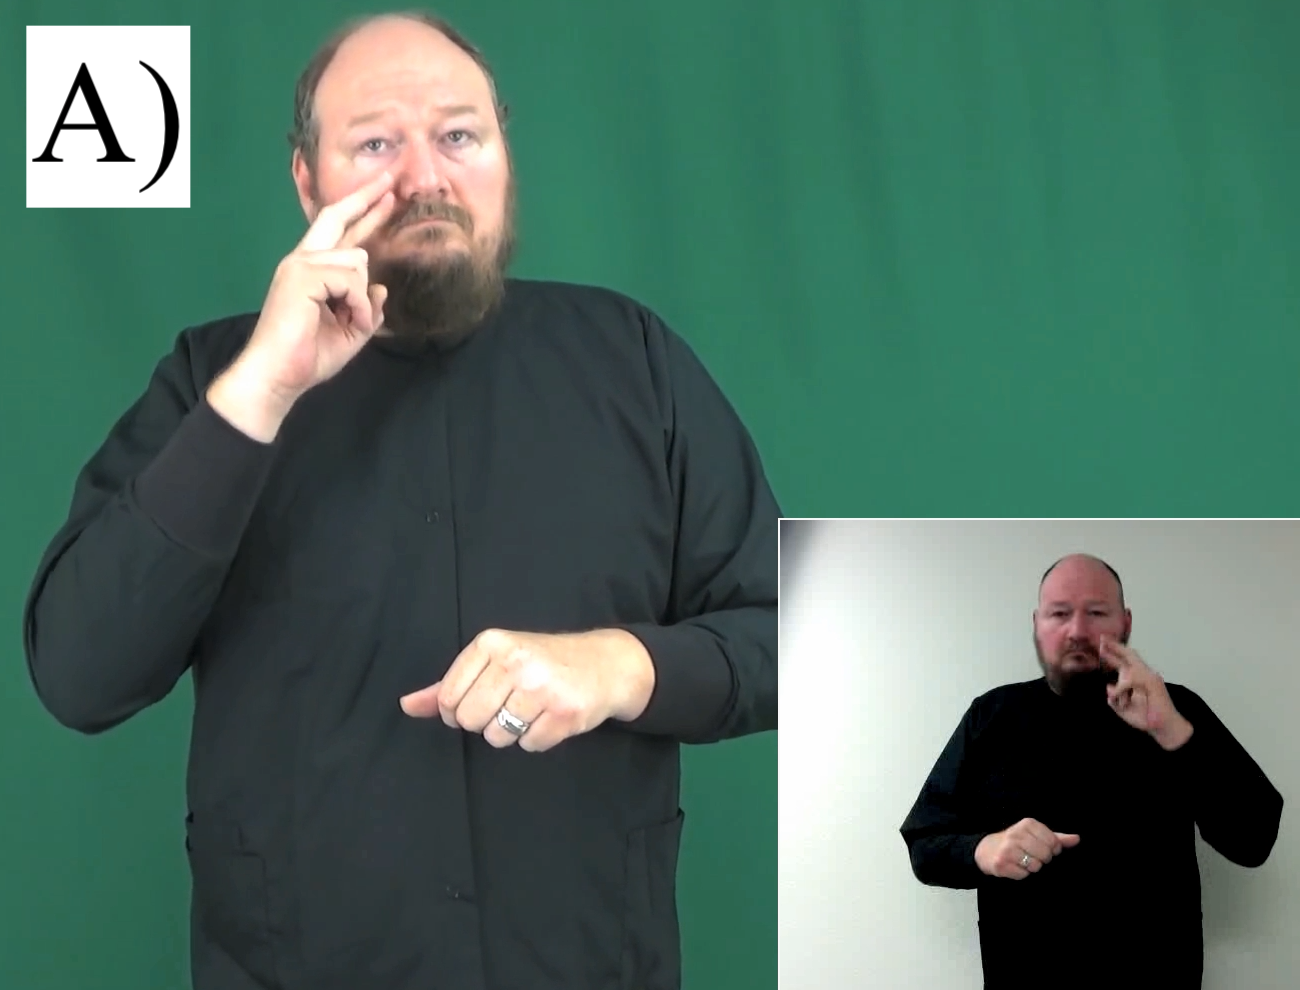
\includegraphics[scale=.15]{SilverSelf} 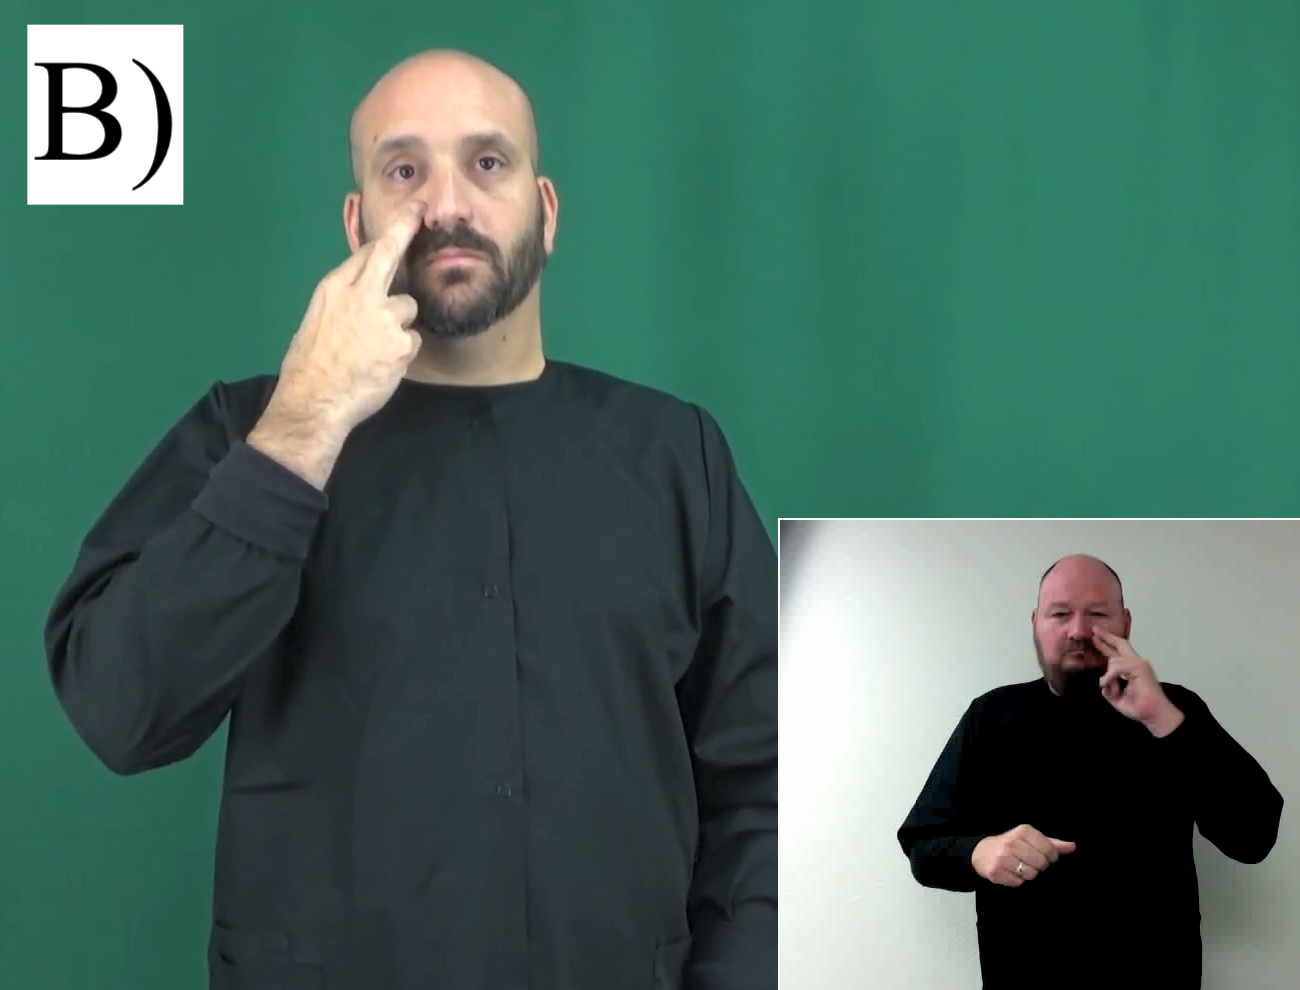
\includegraphics[scale=.15]{SilverFriend}  
                \caption[Silverback\txreg view]{Screenshots from Silverback\txreg, software used for measuring lag time. Shown here, Self (left) and Friend (right) conditions.} \label{fig:silver} 
            \end{figure} 

        \subsubsection{Coding}
            The amount of lag, or delay, between the video recording of the participant and the stimulus presented on the computer screen was labeled for each manual production. More precisely, two coders placed labels on an ELAN\txreg timeline, beginning when the stimulus model contacted the target body location for a given production and ending when the participant also contacted that location. Optimally, coders would label one specific frame in the video when a hand touches the target location. However, this moment of contact may take place between or over the course of two frames. In this case, coders were instructed make inferences about the trajectory of articulators by examining adjacent frames, and mark the contact point as the frame closest to when actual contact likely happened. In absence of any actual contact (i.e., a participant approaches, but never touches contact target location), coders were instructed to mark the apex of a movement, or the first frame when a participant was no longer approaching a location before changing direction.  Two coders were trained on the same sample data such that ratings across both coders could be directly compared. Coders discussed any disagreements of 2 or more frames to refine coding practices before coding experimental data. Inter-rater reliability was calculated from 500 experimental data points. 75\% of annotations were within 1 frame margin of error across all two coders and 97\% were within a 2 frames margin of error. \par
            Coders were also instructed to label lag times that contained phonological errors or otherwise did not reflect the participant’s shadowing ability. Of more than 24,000 data points, only 335 were rejected as error. Sixty-three of these were due to an error in the stimulus or technical difficulty. Sixty-five were due to the participants' failure to shadow, whether through a failure to follow instructions or distraction. In forty-four cases, the participant produced a non-target item (i.e., rather than producing grooming gesture Scratch Face, the participant produced Scratch Head). One hundred forty-one errors were phonological: handshape, location or movement. The majority of phonological errors were in location (\i{n} = 85), followed by handshape (\i{n} = 49), and movement (\i{n} = 7). These errors are excluded from the following analyses.  For each phonological error type, nonsigners showed a greater number of errors than their signer counterparts. The only category where signers exhibited greater number ‘errors’ was in technical issues.\par 
    \subsubsection{Analysis}
                The shadowing dataset was analyzed to address two distinct groups of hypotheses. The first analysis examined the role of model identity (Self, Friend or Other) as it relates to either egocentric bias or visual familiarity, the second analysis addresses hypotheses related to production symmetricity and both analyses address hypotheses related to the role of language experience in phonological predictive representations.  Statistical analyses were conducted with Stata 14.2 \cite{stata14}. Both tests are linear mixed effects models, with post-estimation contrasts of marginal linear predictions. \par     
    \subsection{Results}
        % Intro
        \subsubsection{Effect of Model}
            To examine the role of model identity in predicting lag time, a Model, Group, Type, and all interactions thereof were included as fixed factors in the prediction of lag times. Condition order, an ordinal variable ranging from one to six, item identity, and subject were included as random intercepts. Finally, both Action Type and Model relationship were included as random slopes relative to the subject intercept. In essence, this model focuses on a full factorial design of Type, Model and Group, while parsing out variation due to order effects, or variation in difficulty between items. Random slopes of conditions relative to subject allow for between subject variation in effect of conditions of interest. One subject, for example, showing a huge contrast between grooming gesture and pseudosign, will not sway the overall analysis. \par

 

            \begin{table}[!h]\centering \begin{threeparttable}
                \caption[Shadowing effect of Model, mixed effect model]{Summary of effect regressions of Lag times across the fixed factors (Model, Action Type and Group), and their interactions.} \label{tab:shad_lme_ego} %Table_Shad_Ego_LME.tex 
\begin{tabular}{lrrrr}
\toprule  
& \multicolumn{1}{c}{Coefficient} & \multicolumn{1}{c}{\i{SE}} & 
\multicolumn{1}{c}{\i{z}} & \multicolumn{1}{c}{\i{p} $> |$\i{z}$|$}
\\ \midrule
\multicolumn{5}{l}{Fixed Effects} \\
\IE Intercept & 448.101 & 20.173 & 22.21 & $<$ 0.001\\ %&\thrS\\
\IE Group & 15.784 & 28.171 & 0.56 & 0.575\\
\IE Model & & & & \\
\IE\IE Self vs. Friend & 20.158 & 7.299 & 2.76 & 0.006\\ %&\twoS\\
\IE\IE Self vs. Other & 24.685 & 11.151 & 2.21 & 0.027\\ %\oneS\\
\IE Group * Model & & & & \\
\IE\IE Self vs. Friend & -10.710 & 10.204 & -1.05 & 0.294\\
\IE\IE Self vs. Other & -10.330 & 15.538 & -0.66 & 0.506\\
\IE Type & 30.055 & 15.819 & 1.90 & 0.057\\ %&\marS\\
\IE Group * Type & -44.825 & 22.094 & -2.03 & 0.042\\ %\oneS\\
\IE Model * Type & & & & \\
\IE\IE Self vs. Friend & -17.179 & 7.778 & -2.21 & 0.027\\ %&\oneS\\
\IE\IE Self vs. Other & -22.385 & 7.842 & -2.85 & 0.004\\ %&\twoS\\
\IE Group*Model & & & & \\
\IE\IE Self vs. Friend & 20.575 & 10.870 & 1.89 & 0.058 \\ %\marS\\
\IE\IE Self vs. Other & -7.850 & 10.916 & -0.72 & 0.472\\
\multicolumn{5}{l}{Random Effects} \\
\IE Subject & & & & \\
\IE\IE \i{SD} (Intercept) & 7360.171 & 1766.465 &   & \\
\IE\IE \i{SD} (Type) & 4006.918 & 1018.044 &   & \\
\IE\IE \i{SD} (Model) & 441.42 & 120.056 &   & \\
\IE \i{SD} (Item) & 1042.484 & 114.318 &   & \\
\IE \i{SD} (CondOrder) & \multicolumn{2}{c}{NA\tnote{a}} &   & \\
\bottomrule
\end{tabular} 
\begin{tablenotes}
    \small
      \item \i{Note}. \i{SD} = Standard Deviation; \i{SE} = Standard Error; \i{p} = p-value significance; CondOrder = Order of Condition; NA = Not available. \item[a] Calculation suppressed due to computational limitations.
      %\item \oneS \i{p} $<$ .05, \twoS \i{p} $<$ .01, \thrS \i{p} $<$ .001.  
      \end{tablenotes}  
            \end{threeparttable} \end{table}
            



 

            \begin{figure}[!h] \centering 
                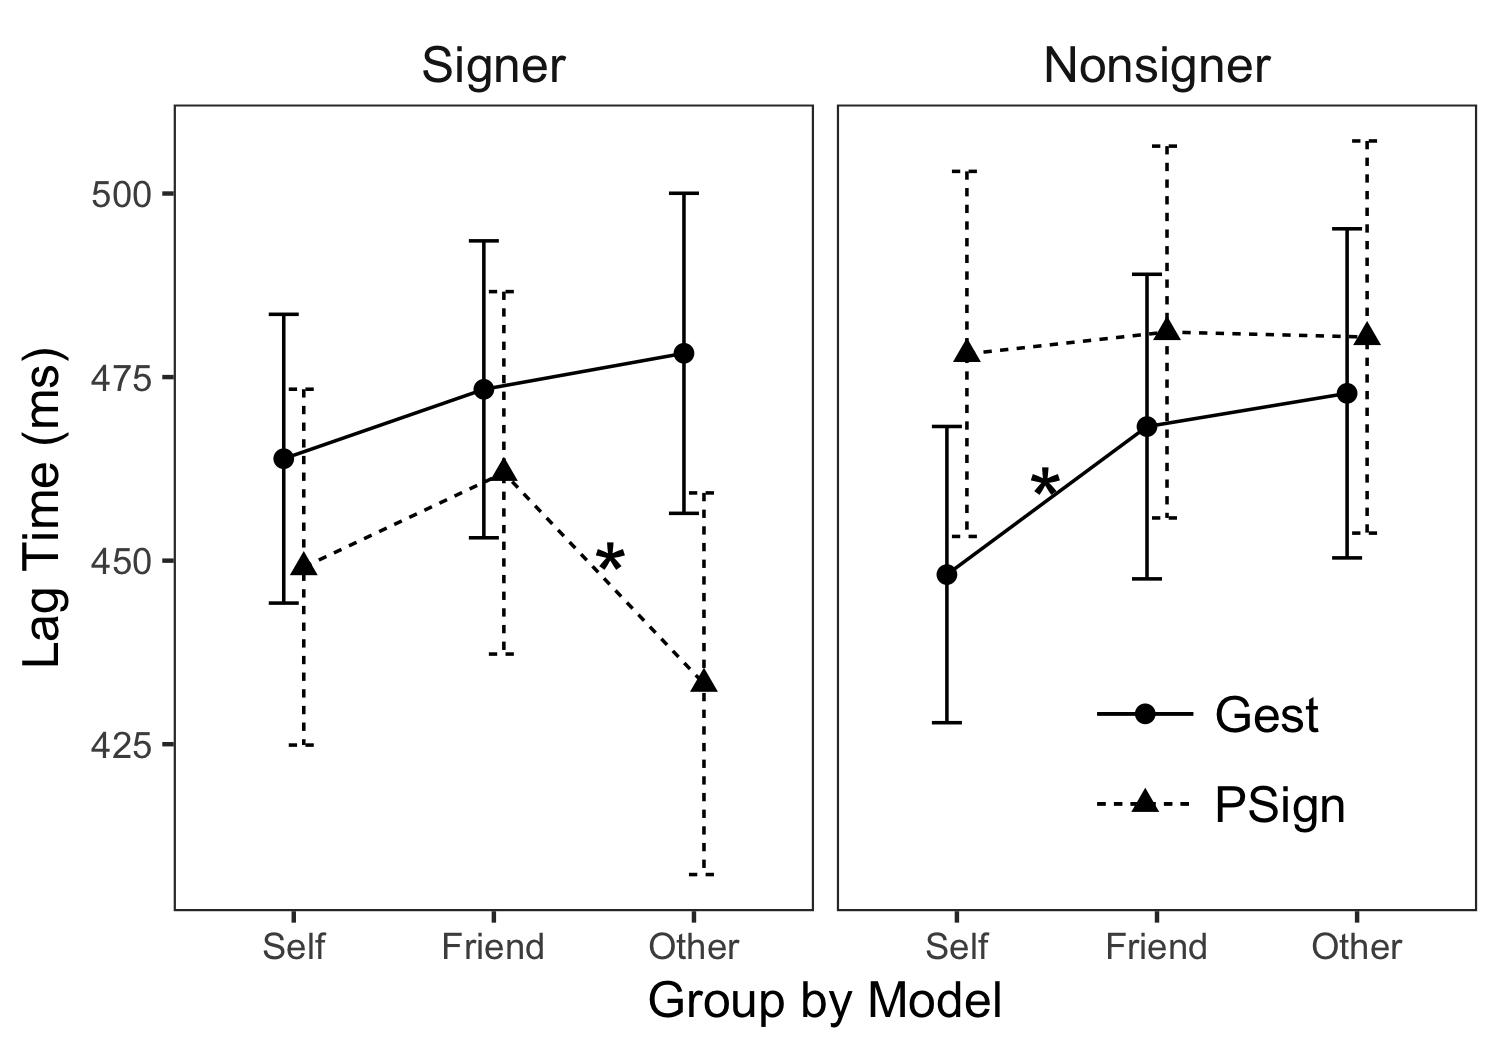
\includegraphics[scale=\sc]{Fig_Shad_Ego.png} 
                \caption[Parameter estimates: Shadowing, effect of Model]{Parameter estimates for a linear mixed effects model examining the effect of Model and Type (Gest = grooming gesture; PSign = pseudosign) on lag times for each group.} \label{fig:shad_ego}
            \end{figure}
            The omnibus test of this model is shown in Table \ref{tab:shad_lme_ego} and parameter estimates for each condition are shown in Figure \ref{fig:shad_ego}. Counter to expectations, there was no main effect of Group. There were, however, main effects of Model, as well as a marginal main effect of Type. There was a significant two-way interaction between Group and Action Type, \i{p} = 0.042. Parameter estimates indicated a trend whereby nonsigners showed faster lag times for grooming gestures compared to pseudosigns (\i{M} = 463, \i{SE} = 20.5; \i{M} = 480, \i{SE} = 25.1), while signers showed slower lag times for grooming gestures compared to pseudosigns (\i{M} = 472, \i{SE} = 20.0; \i{M} = 448, \i{SE} = 24.5). A contrast of marginal linear predictions showed no simple effects: neither group showed a significant difference between Action Type. Simple effects were only seen by testing at each level of Model for each group: nonsigners showed a marginal Type difference for Self stimuli, \chsq(1) = 3.61, \i{p} = 0.057, and signers showed a significant Type difference for Other stimuli, \chsq(1) = 8.52, \i{p} $<$ 0.01. This two-way interaction is instead better understood within the context of the three-way interaction of Group, Type and Model. \par
            In the omnibus test, there was a marginal three-way interaction between the first two levels of Model (Self and Friend), Type and Group, \i{p} = 0.058. Contrasts of marginal linear predictions were performed to test hypotheses regarding egocentric bias (Self vs. Friend) and visual familiarity (Friend vs. Other). Nonsigners exhibited an interaction between Type and the Self vs. Friend model contrast, \chsq(1) =  4.88, \i{p} =0.03. Signers showed no such interaction, \chsq(1) =  0.20, \i{p} =0.65. An additional contrast to parse this two-way interaction showed that nonsigners exhibit an egocentric bias for grooming gestures, \chsq(1) = 7.63, \i{p} = 0.01, but not pseudosigns, \chsq(1) = 0.17, \i{p} = 0.68. Nonsigners were significantly faster for grooming gestures when shadowing themselves (\i{M} = 448, \i{SE} = 20.2) compared to their friend (\i{M} = 468, \i{SE} = 20.7).\par
            Regarding the effect of visual familiarity, there was a three-way interaction between model (Friend vs. Other), type and group, \chsq(1) = 6.80, \i{p} = 0.01. Examining this as a two-way interaction for each group revealed that the signers showed a visual familiarity effect, \chsq(1) = 19.62, \i{p} $<$ 0.01, but the nonsigners do not, \chsq(1) = 0.44, \i{p} = 0.50. Further investigation revealed that this effect is present in the pseudosign stimuli, \chsq(1) = 16.24, \i{p} $<$ 0.01, but not the grooming gestures, \chsq(1) = 0.47, \i{p} = 0.49. Contrary to expectations, signers were significantly slower when shadowing their friend (\i{M} = 462, \i{SE} = 24.7), compared to the unknown Other model (\i{M} = 433, \i{SE} = 26.0).\par
            One way to understand the anti-familiarity effect among the signers is to assume that there is something about the pseudosign stimuli that were inherently more predictable in some pragmatic way. One means of making a stimulus more predictable is to have a more stable inter-item interval (i.e., a more regular beat or rhythm). Measures of inter-item intervals were available because Chapter \ref{ch:trans} measured transition times for all 96 target items within the Other model’s videos. With 48 items per Action Type, a post-hoc paired t-test showed that grooming gesture transition times (\i{M} = 1106, \i{SD} = 416) were significantly faster than pseudosign transition times (\i{M} = 1242, \i{SD} = 361), \i{t}(47) = -2.58, \i{p} = 0.01. An extra 100ms may be enough to give signers an advantage in these predictions, but variance (as opposed to duration) is a better representation of temporal regularity. Variance refers to how tightly data points are clustered around the mean. A smaller variance in transition duration would mean that items were produced at a more regular interval. A post-hoc F test of equality of variance indicates that there is no significant difference between the regularity of pseudosign and gesture productions in the Other stimuli, \i{F}(1,47) = 1.33, \i{p} = 0.17. \par
        \subsubsection{Effect of Symmetricity}
            A very similar model to the one described in the previous section was used to examine the effect of Symmetricity (one- vs. two-handed) items on lag time. The only difference between this model and the previous one is that model was exchanged for Symmetricity as both a fixed factor and a random slope. Fixed factors included Symmetricity, Type, Group, and all interactions. Random intercepts included item, condition order, and subject, with subject by Type and subject by Symmetricity random slopes. Random intercepts permit variation in overall lag time depending on item or the order of the condition. Random slopes permit lag time variation in how each subject exhibits Action Type or Symmetricity effects, while still looking at these effects across the dataset. \par
            
            \begin{table}[!h]\centering \begin{threeparttable} 
                \caption[Shadowing effect of Symmetricity, mixed effect model]{Summary of effect regressions of Lag times across the fixed factors (Symmetricity, Action Type and Group), and their interactions.} \label{tab:shad_lme_sym}
                %Table_Shad_LME_Sym.tex 
\begin{tabular}{lrrrr}
\toprule  
& \multicolumn{1}{c}{Coefficient} & \multicolumn{1}{c}{\i{SE}} & 
\multicolumn{1}{c}{\i{z}} & \multicolumn{1}{c}{\i{p} $> |$\i{z}$|$}
\\ \midrule

\multicolumn{5}{l}{Fixed Effects} \\
\IE Intercept & 469.574 & 20.922 & 22.44 & $<$ 0.001\\
\IE Group & -2.624 & 29.209 & -0.09 & 0.928\\
\IE Sym  & -12.598 & 6.553 & -1.92 & 0.055\\
\IE Group * Sym & 22.282 & 9.114 & 2.44 & 0.014\\
\IE Type & -2.353 & 15.816 & -0.15 & 0.882\\
\IE Group * Type & -25.767 & 22.066 & -1.17 & 0.243\\
\IE Sym * Type & 38.502 & 8.64 & 4.46 & $<$ 0.001\\
\IE Group * Sym * Type & -29.47 & 12.005 & -2.45 & 0.014\\
\multicolumn{5}{l}{Random Effects} \\
\IE Subject & & & & \\
\IE\IE \i{SD} (Intercept) & 7962.053 & 1900.127 &  & \\
\IE\IE \i{SD} (Type) & 4042.037 & 1022.397 &  & \\
\IE\IE \i{SD} (Sym) & 108.194 & 107.688 &  & \\
\IE \i{SD} (Item) & 755.736 & 113.81 &  & \\
\IE \i{SD} (CondOrder) & \multicolumn{2}{c}{NA\tnote{a}} &   & \\
\bottomrule
\end{tabular} 
\begin{tablenotes}
    \small
      \item \i{Note}. \i{SD} = Standard Deviation; \i{SE} = Standard Error; \i{p} = p-value significance; Sym = Symmetricity; CondOrder = Condition order, first through sixth. \item[a] Calculation suppressed due to computational limitations. \end{tablenotes}
            \end{threeparttable}\end{table}
            \begin{figure}[!h] \centering 
                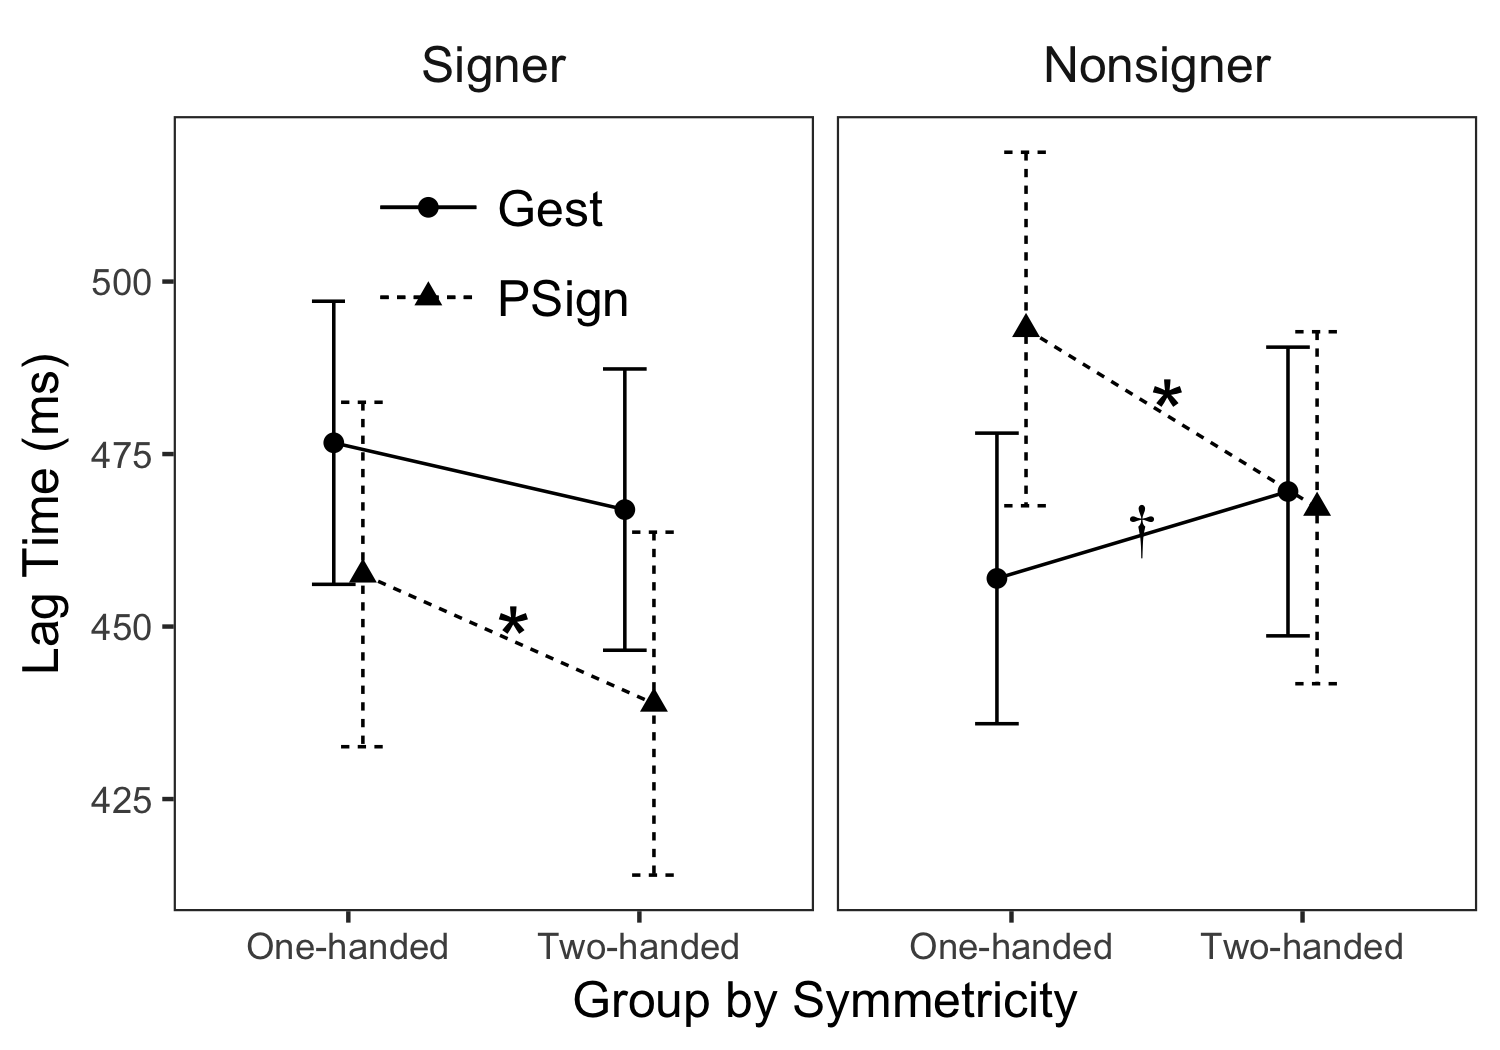
\includegraphics[scale=\sc]{Fig_Shad_Sym.png} 
                \caption[Parameter estimates: Shadowing, effect of Symmetricity]{Parameter estimates for a linear mixed effects model examining the effect of Symmetricity and Type (Gest = grooming gesture; PSign = pseudosign)  on lag times for each group. \marS \i{p} $<$ .1, \oneS \i{p} $<$ .05.} \label{fig:shad_sym}
            \end{figure}    
 
 

            The omnibus test of this model is shown in Table \ref{tab:shad_lme_sym} and parameter estimates for each condition are shown in Figure \ref{fig:shad_sym}. Consistent with the previous model, but counter to predictions, there was no main effect of Group. There was, however, a marginal main effect of Symmetricity, \i{p} = 0.055, whereby one-handed items had marginally longer lag times (\i{M} = 471, \i{SE} = 15), compared to two-handed items (\i{M} = 460, \i{SE} = 15). There was also a two-way interaction between Group and Symmetricity, \i{p} $<$ 0.05, and contrasts of marginal linear predictions indicate that signers exhibit a main effect of Symmetricity, \chsq(1) = 8.85, \i{p} $<$ 0.01, but nonsigners do not, \chsq(1) = 1.82, \i{p} = 0.18. Again, this two-way effect can be better understood in the context of the three-way interaction. \par
            The omnibus test of the model showed a three-way Symmetricity by Type by Group interaction, \i{p} = .01. Contrasts here revealed that nonsigners exhibit a two-way interaction between Symmetricity and Type, \chsq(1) = 19.86, \i{p} $<$ 0.01, but this was not the case for signers, \chsq(1) = 1.17, \i{p} = 0.27. Further, nonsigners showed a significant effect of Symmetricity for pseudosigns, \chsq(1) = 15.56, \i{p} $<$ 0.01, and a marginal effect of Symmetricity for grooming gestures, \chsq(1) = 3.70, \i{p} = 0.055. An examination of parameter estimates revealed that these effects were in opposite directions. For pseudosigns, nonsigners showed significantly faster lag times for two-handed items compared to one-handed items (\i{M} = 457, \i{SE} = 21.1 vs. \i{M} = 470, \i{SE} = 20.9). For grooming gestures, nonsigners showed marginally slower lag times for two-handed items compared to one-handed items (\i{M} = 467, \i{SE} = 25.5 vs. \i{M} = 493, \i{SE} = 25.6).             
    \subsection{Discussion} \label{sec:shad_disc}
        %
            Through the first model, presented in Table \ref{tab:shad_lme_ego}, we can see that the signers and nonsigners shadow the grooming gestures and pseudosigns differently. Although parameter estimates (a) are in line with predictions about signers showing shorter lag times for more familiar sign phonology and (b) point to improved prediction abilities for more familiar grooming gestures for nonsigners, these trends are only visible as an interaction between group and linguistic status rather than strong preferences in for either stimulus type within either group. Instead, the trends (a) and (b) are driven by differential responses for specific models. Signers show significantly better pseudosign predictions abilities for the well-trained unfamiliar model, when compared to grooming gestures performed by the same model. Nonsigners show significantly better grooming gesture prediction abilities for themselves, when compared to predicting their own pseudosign productions. Although these trends can be described as in support of hypotheses regarding the effect of phonological knowledge or perceptual familiarity of grooming gestures, the pattern of results is better explained through differences related to egocentric bias or prosodic cues. \par
            The contrasting models in the present experiment were, in part, presented to look for direct evidence of egocentric bias in each group, for each stimulus type. Under the conditions that most closely replicate previous studies \cite<e.g.,>[]{knoblich2001}, with nonsigner participants watching familiar stimuli (i.e., grooming gestures), in a comparison between oneself and one's friend, there was evidence of egocentric bias. The lack of evidence of egocentric bias for nonsigners shadowing pseudosigns is harder to explain. The nature of motoric simulation in the context of \citeA{PG} requires that the predicted actions be sufficiently familiar in order to generate a motor command from perception alone. It may be the case that nonsigners’ dearth of pseudosign experience leaves them incapable of accessing the motor commands required for covert imitation. However, the lesson regarding egocentrism from both \citeA{watkins2017} and \citeA{hickok2011} was that covert imitation facilitates predictions for particularly difficult stimuli. Overall means indicate that pseudosign stimuli were more difficult for the nonsigners than grooming gestures, there was no egocentric bias for the more difficult pseudosigns. Instead, the present evidence may point to a revision of Hickok’s (2011) proposal, whereby difficult \i{but familiar} contexts engage motor simulation. \par
            Hickok’s (2011) notion that only particularly difficult stimuli engage motor simulation is especially relevant for examining signer shadowing performance. It may be the case that sign language experience renders shadowing a less cognitively demanding task for the signers compared to nonsigners. Additional correlation evidence from Experiment 4 points to this being the case. For signers, documented egocentrism effects in \citeA{watkins2017} were limited to two-handed asymmetrical items, which were not present in the present study. Future Shadowing studies might include more complex stimuli such as this.\par
            Friend versus Other contrasts were performed on the relevant mixed effects model (see Table \ref{tab:shad_lme_ego} for model information) to examine the effect of visual familiarity on shadowing ability. No facilitative effect can be seen. Instead, signers were significantly faster for the unknown Other model when shadowing pseudosigns compared to shadowing Friend. This finding has greater bearing on the quality of these stimuli than on the nature of shadowing familiar versus unfamiliar models. The quality of Friend stimuli was restricted as it reflected the best productions that participants (both signer and nonsigner) could produce in the limited span of an hour and fifteen minutes. In contrast, the Other model was a dedicated hearing signer confederate who was more highly trained over the course of several hours. While the average participant developed no memory for the randomized order of each string in their limited viewings, the Other model memorized these lists to some extent. The Other model may have, therefore, provided higher quality, and therefore more predictable productions. In this case, quality could refer to either (a) the features of a good production that were explicitly solicited from participants or (b) phonological or prosodic regularities of the sort seen in natural sign language production. \par
            In the former case, high quality productions were experimentally defined as having few hesitations and disfluencies (i.e., pauses or the manual equivalent of ‘umm’) as well as productions closer to the target handshape, location, and movement. If this pattern was simply an effect of increased fluidity and more consistency, yielding more predictable stimuli, one would expect to see a shorter lag times for Other across groups and stimulus types. Instead, this benefit was only observed for the signers shadowing pseudosigns. Therefore, there may be some prosodic feature of the Other model’s pseudosign productions that were inherently more predictable only by those with sign language experience interpreting such prosodic cues. In other words, the Other model (a highly proficient signer), knowing she was producing pseudosigns, may have applied prosodic cues to these stimuli and not the gestures, which were, in turn, only interpretable to those familiar with interpreting such prosodic information. \par
            It is difficult, however to specify exactly what these prosodic cues may be. Subtleties in the location of the hands for a given item can impart information about future locations via co-articulation \cite{grosvald2012,mauk2003} and, while signers can glean important information from handshape transitions during fingerspelling \cite<Schwarz, 2000; as cited in>[]{geer2017}, the same information may be distracting to nonsigners \cite{geer2014}. The Other model often knew what the next pseudosign would be, as a result of more extensive training, and may have provided subtle co-articulation as prosodic cues across location, handshape and movement. She may have, for example, produced pseudosigns at the face slightly lower if the subsequent item were produced in neural space. Considering the stimulus, it is possible that the Other model only produced co-articulation in her pseudosign videos and not in her grooming gestures. Considering group differences, these co-articulatory cues may only be predictively useful for signers. Even if the same cues were present in the grooming gesture videos, it is possible that signers only considered co-articulation information relevant in linguistic contexts. Sign language comprehension, in general, makes use of manual co-articulation to facilitate phonological forward models \cite{grosvald2012}, but evidence of group differences in this domain, while intuitive, have yet to be demonstrated. The present data cannot, however, differentiate between this information being only present in phonological contexts versus being only perceptually useful in these contexts. 
            A prosodic cue that was measured is temporal regularity; items produced with a regular rhythm may be more predictable than those produced with a more random interval. This information is, in part, available through measurements made for experimental targets used Experiment 2. Specifically, 96 inter-item intervals were measured in these videos. Transition time between items was approximately 100ms longer for the Other model’s pseudosigns compared to her grooming gestures. These two means are not statistically different in their variance, however, indicating that the pseudosigns were not significantly more regular in their timing. With only 48 observations per Type, this test may have been underpowered, but future investigations might examine what specific prosodic cues make stimuli more predictable. The prosodic differences across pseudosign and grooming gesture strings for the Other model may be subtler than duration or co-articulation. There may be differences, for example, in the acceleration profiles of transition movements. The next section will go in more detail regarding the role transitional information may play in facilitating predictions. \par
            A separate statistical model in the present experiment addressed the effect of symmetricity, as inspired by the notion that non-dominant hand activation may be difficult to suppress, and particularly difficult for nonsigners. Contrary to expectations, signers showed slightly longer lag times for both one-handed grooming gestures and pseudosigns. While this non-dominant hand suppression can be seen in pseudosign shadowing lag times for the nonsigners (longer for one-handed pseudosigns), nonsigner grooming gesture lag times showed the opposite effect. For nonsigners, it was marginally easier to shadow one-handed grooming gestures compared to two-handed grooming gestures. This is a difficult effect to explain in isolation, but it does fit into a broader pattern. \par
            Specifically, for signers, symmetricity has the same effect across Action Types; signers are treating all stimuli similarly. This result suggests that sign language experience may have guided how these participants approached this task more broadly. Regardless of stimulus type, pseudosigns or grooming gesture, signers show trends toward facilitation of symmetrical productions. Nonsigners, in contrast, only show symmetrical facilitation for unfamiliar and phonologically complex pseudosigns. Nonsigners were marginally faster for one-handed familiar grooming gestures. It may be the case that one-handed grooming gestures are more familiar to nonsigners than the two-handed counterparts, as these one-handed items may be more frequent in day-to-day use. When considered in tandem with egocentric bias (self vs. friend) results discussed above, it may be the case that a very detailed egocentric motoric simulation guides nonsigner shadowing of grooming gesture: when stimuli are familiar, nonsigners can draw directly from their own experiences and ease of one-handed gesture production. Nonsigner motoric simulation of pseudosigns, in absence of detailed motor experience, may be more abstract and more susceptible to broad motor effects like non-dominant hand suppression. \par
            Overall, the present Experiment does little to support the Pickering and Garrod (2013) model of persistent and robust motor simulation. The limited evidence of egocentric bias presented here instead recalls proposals related to familiarity biases \cite{watkins2017} and cognitive load \cite{hickok2011}. Pseudosigns were insufficiently familiar for the nonsigners to engage in egocentric motor simulation, and shadowing broadly may not have been sufficiently cognitively demanding to solicit such and effect for the signers. Where there is egocentric bias, however, in nonsigner grooming gestures, there is also evidence for familiarity facilitation of one-handed gestures. Where there is a lack of egocentric bias, in signer shadowing, there is evidence of difficulty suppressing motor activity on the non-dominant hand, despite hypothesis regarding the modulating influence of sign language experience on suppression abilities. Instead, signers’ relative ease in shadowing a skilled signer model highlights the need for future research on the phonological or prosodic cues that might lead to such facilitation\footnote{This chapter, in part, is currently being prepared for submission for publication of the material. Brozdowski, Chris; Emmorey, Karen. The dissertation author was the primary investigator and author of these materials.}. 

\section{Experiment 2: Transition motion in manual predictions}
    \label{ch:trans}
    \subsection{Introduction} 
        %%
            The present Experiment was designed to build upon notions of predictive representations, as investigated in Experiment 1. While Experiment 1 was focused on the mechanisms that facilitate predictive representations (i.e., motoric simulation and familiarity) for the individual, Experiment 2 is more focused on the nature of the stimulus and, more specifically, the phonological parameters available during transitional periods. After defining what is meant by a transition, the present introduction will provide evidence that signers use these periods to generate predictive models of linguistic stimuli, and set up questions regarding the utility of handshape versus movement during these periods, as well as the transferability of these abilities outside linguistic contexts. \par
            For the purposes of the present discussion, the transitional period was defined by \citeA{jantunen2013}. This period begins as soon as the dominant hand diverts from the movement specified by a given pseudosign or grooming gesture. The transitional period ends immediately prior to the specified movement for the subsequent item. Using this demarcation method, \citeA{jantunen2013} examined fluid narrative signing and found differences between signs and transitions in both speed and acceleration profiles. While there is some debate in the literature as to the length of signs or how to divide up fluid signing \cite<see>[]{jantunen2015}, \citeA{jantunen2013} makes the case that there is a qualitative phonological difference between signs and transitions. \par 
            When viewed through this lens, existing evidence on sign perception indicates that transitional periods facilitate predictive models. \citeA{hosemann2013} presents evidence that signers are able to detect a semantically anomalous sign slightly prior to onset. \citeA{arendsen2007} presents evidence that, for signers, links longer transition lengths to shorter reaction times in a sign identification task. For participants in each study, the information immediately prior to sign onset was likely somehow incorporated into predictive representations. More remains to be asked, however, about what components of transitional information are useful to signers. The components of the signal can be broken down by phonological parameter: movement, or trajectory, and handshape. Each could theoretically contribute to predictions in comprehension as the signer transitions from one lexical item to the next. \par
            The direction of broad transition movements would allow a signer to draw conclusions about the onset location of a subsequent sign. For example, a hand moving upward at high velocity could probabilistically give information about an onset location at the forehead for the subsequent sign. A slower velocity might signal the next onset location as the chin. By narrowing the possibility space for subsequent location, a signer would be more rapidly able to activate the relevant sign. While there is currently evidence for co-articulation in sign \cite<e.g.,>[]{mauk2003}, the only evidence that comprehenders can make use of these cues focuses on anticipatory location co-articulation on a previous sign, and demonstrated that, with explicit instruction, both signers and nonsigners are capable of detecting this cue \cite{grosvald2012}. No such evidence for the utility of transitional velocity exists. \par
            By analogy to spoken language, however, we can see a process similar to the proposed utilization of velocity occurring with phonological onset competitors in eye-tracking research \cite<e.g.,>[]{allopenna1998}. Here, spoken language users listen to a target word and activate non-target items with the same phonological onset. Given a high, as opposed to low, velocity transition upward, an experienced signer might activate a set of signs in a high location phonological neighborhood. Experiment 2 examined to what extent signers and nonsigners rely on transitional movement in predictive contexts, and whether or not signers' ability to attend to transitional movement is confined to contexts with sign phonology.  \par
            During the course of transitional movements, the shape of the hand also changes. Much in the same way as signers likely use movement to draw inferences about the phonological onset of the upcoming sign, signers may use pre-onset handshapes to generate predictive representations about the handshape of a subsequent sign. There are even some instances in ASL when signers must attend to intermediate handshapes. \i{Fingerspelling} refers to the rapid sequential presentation of signs that correspond to letters in an orthography, and is used by ASL signers to refer to proper names in English, for example. In ASL, these letters are primarily unique handshapes. While rapid transitions between handshapes alone are not sufficient information for comprehending, signers do make use of this information in fingerspelling comprehension \cite<Schwarz, 2000, as cited by>[]{geer2017}. \par
            Additionally, when specific words are produced frequently, certain fingerspelled words are start to lexicalize in order to to better conform to the phonology of ASL \cite{cormier2008, brentari1998}. This lexicalization process can include dropping some letters or not fully articulating others in order to conform to phonological constraints or improve efficiency. Because signers extract intermediate handshapes in comprehending natural fingerspelling, they may be better equipped to generate predictive representations based on handshape information prior to the onset of a sign. The present Experiment examined whether or not singers and nonsigners differ in their ability to incorporate transitional handshapes into predictive representations, as well as whether or not this ability to attend to transitional handshape is confined to contexts with sign phonology. \par
            To examine participants' ability to attend to both transitional movement and handshapes, Experiment 2 selectively degrades transitional information in different ways, while preserving the timing of presentation. First, the sentence-like strings of Other model videos, as described in Experiment 1, are used in Experiment 2 as \i{Normal} videos. Second, \i{Blur} videos were generated by applying a moving Gaussian blur to only to the hands in the Normal videos during all transitional periods. This blur eliminated all transitional handshape information. \i{Hold} videos took the final frame of the immediately prior to a transition and extended its duration for the entire transitional period. Each Hold video began with the model in the rest position until the first frame of the first item. The video then froze on the final frame of each item. The frozen frame lasted for the duration of each transitional period. Participants watched these videos monitoring for a target item that may occur at any point. While this response-to-target procedure does not rely on overt imitation of the stimulus like shadowing in Experiment 1, participants were expected to provide response times consistent with the strength of their predictive representations. The stronger a predictive representation, the faster a participant can identify a target stimulus. \par
            These predictions, as proxy for forward models, are hypothesized to play a major role in language comprehension \cite{PG}. By extension, it was hypothesized that sign language experience would bolster motoric predictive representations, and therefore predicted that signers would have overall faster response times compared to the nonsigner group. As previous evidence points to signers making use of transitional movement \cite{arendsen2007, hosemann2013} and handshapes \cite{brentari1998, cormier2008} during language comprehension, it was further predicted that signers would show greater RT penalties due to the loss of transitional information (i.e. slower RTs for Blur compared to Normal videos and slower RTs for Hold compared to Blur videos). 
            The present Experiment maintains the same one- vs. two-handed stimuli as Experiment 2. In the context of the broader work, via evidence of the difficulty and additional neural activation associated with producing asymmetrical signs \cite{meier2006, hickok1996, emm2016}, one-handed production and motor simulation are hypothesized to require non-dominant hand suppression. Under Pickering and Garrod's (2013) proposal, covert motor simulation guides predictive abilities such as those required to perform the present response to target task. As such, predictions regarding Symmetricity contrasts, as described on page \pageref{par:sym_hyp}, were predicted to hold across both Experiments. Namely, sign language experience was expected to grant users improved ability to suppress non-dominant hand activity, which renders one-handed motor simulations naturally more difficulty than symmetrical two-handed simulations. Nonsigners were expected to show increased RTs for one-handed productions and signers were expected to show reduced or no difference between one- vs. two-handed items, as a result of greater experience suppressing non-dominant hand activity. \par
            This is not to say that the two experiments are exactly the same, however. While Shadowing requires full overt production in addition to motor simulation, the present Experiment only requires the latter. As such, a reduced effect of Symmetricity, relative to the previous Experiment, was predicted. Alternatively, it may be the case that motor simulation is not engaged by a more passive button-press task. Such a task is more susceptible to visual matching strategies, and maintaining one’s hand on a button may be sufficient to suppress dominant hand motor simulation. Evidence from symmetricity contexts across the two Experiments is contrasted in Section \ref{sec:disc_sym} of the General Discussion.\par
    \subsection{Methods}
        \label{sec:trans_meth}
        \subsubsection{Participants}
            Forty-two right-handed participants were recruited from the community in San Diego via fliers, online postings, and word of mouth. Twenty-one Deaf signers (13 Female, \i{M} age = 35.5, range: 60 to 17, \i{SD} = 9.8), with either early or native sign language exposure (age of acquisition $<$ 6), and 21 sign-na\"ive English speakers (12 Female, \i{M} age = 29.0, range: 19 to 59, \i{SD} = 11.2) participated. In a two-tailed independent samples t-test, signers were found to be marginally older than their nonsigner counterparts, \i{p} = 0.053. This was not considered an issue, however, because all predictions focus on improved reaction times for signers, and age, in general, reduces response times \cite{der2006}. This age differences only contributes to Type II error. Nonsigners had no sign experience or minimal sign knowledge (e.g., a few signs or the fingerspelled alphabet). In parallel with Experiment 1 above, group sizes were selected to roughly match the number of data points per condition present in \citeA{mitterer2008}. \par
        \subsubsection{Design/Materials} 
            Participants saw six conditions in a 3 x 2 design: Condition (Normal vs. handshape Blur vs. Held transitions) by stimulus Type (gesture vs. pseudosign). The timing of videos was never manipulated; the delay between the first and second item in any given string is preserved across conditions. The Normal videos were identical to the Other videos from Experiment 1. The Blur videos added a heavy Gaussian blur to the hands during transitional periods for the same videos. Blurring prevents the use of intermediate handshape in facilitating predictions about the upcoming pseudosign/gesture, while still revealing broader movements of the sort shown in \citeA{klima1999}. The Hold condition preserved the final frame of a pseudosign or gesture for the entire transition time, which removed all transitional information. To the observer, this manipulation appears to be rapid sequential presentation of stimulus items with a still frame in between. Blur and Hold stimuli were generated with Adobe\txreg  Premiere Pro CC. Blur videos were generated by adding a masked blur layer that was key-framed to fit precisely over the hand. All stimuli were shown at 1920 by 1080 pixel resolution, at 60 frames per second. \par
        \subsubsection{Procedure}
            Each participant sat in front of an iMac running OSX 10.8 running Psyscope X B77 \cite{psyscope}. Instructions and practice items demonstrated the structure of this response-to-target task. The instructions were as follows: \par
            \begin{quote}The goal today will be to see how quickly you can identify an invented sign or gesture in context. We will look at this by first showing you a picture of a ‘target’ item. Press the space key to continue to the following video. This video will show several invented signs or gestures in a sequence. Please press the B key as soon as you see the target item. If you forget the picture that was shown, please wait until video ends. If you press the B key and nothing happens, please also wait until the video ends. It's important that you focus and press B as quickly as you can when you see the target item. Sometimes, you will see blurring between invented signs or gestures, or the video will freeze before moving on to the next items. Please do your best to ignore blurring and freezing and only try to predict the target sign or gesture. Let's start with the (pseudosigns/gestures). You will now see a video of each of the possible target items. \end{quote}
            The participant then saw an isolated video of each item of the 12 items in the relevant stimulus Type’s inventory. In each of these sequential demonstration videos, the demonstration model moved from rest position to item to rest position. The participant then saw eight practice trials. For each trial, the participant saw a still frame demonstrating one of the possible target items for that stimulus type. The participant was tasked with pressing a button as soon as they recognized the target within in the video string. Reaction times (RTs) were collected for button-press relative to the onset of the target item. \par
            Each sentence-like string of eight items was shown four times, resulting in 48 RTs per condition and 288 data points per participant. Each of the 24 possible items (see Table \ref{tab:stim} on page \pageref{tab:stim} for details) was shown four times for each of three video conditions and each of two type. \phantomsection\label{par:hs_complexity} These items were matched across pseudosigns and grooming gestures for location. Handshapes in the pseudosign inventory were more complex than those in the grooming gesture. \citeA{brentari1998} uses the linguistic notion of markedness to discuss handshape complexity. Using the Stokoe notation system \cite{stokoe2005}, \citeA{brentari1998}, p.~118, defines the set of unmarked (i.e., less complex) handshapes as B, A, S, C, O, 1 and 5. Three of twelve pseudosigns fit this criterion. While the grooming gestures don’t, in general, map on to sign phonology, their handshapes can be approximated by Stokoe notation. Eleven of the twelve grooming gestures match the criteria for unmarked handshapes \cite{brentari1998}. \par
            The experiment took 30 to 45 minutes to complete. Trials were balanced such that the target was equally likely to occur in any of the eight possible positions within a string (first, second, third, etc.); six items were shown for each position within each condition. On average, the target appeared 5.2 seconds into the video (range: 0.6-11.1s, \i{SD} = 3.1s). Targets were matched across stimulus types (e.g., for grooming gesture string number 1, gesture number 7 was the target in third position, and, for pseudosign string number 1, pseudosign number 7 was the target in third position).\par
            Stimulus type (pseudosign vs. grooming gesture) was blocked and counterbalanced across participants. At the halfway point within each block, as well as between blocks, participants were prompted to take a break. Each quarter of the experiment was designed to have equal numbers of items in each condition, as well as an equal number of one-handed and two-handed items. Items were randomly presented within each quarter. \par
            Subject keypresses were accepted by Psyscope \cite{psyscope} for the entire duration of the video. While subjects were permitted to respond either before or after the onset of the target item, and RTs are measured relative to this onset, efforts were taken to remove any false positives or errant key presses. Responses were labeled as inaccurate if they occurred prior to the transition immediately preceding the target item because a subject cannot identify a target prior to any phonological features being present. A key press was rejected as too late if the response time was greater than two standard deviations above the mean for that specific combination of target, video and language group. Of approximately 16,800 data points, 2,371 or 14.1\% were rejected these grounds. While nonsigners had, on average, more errors than signers, this was not a significant difference, \i{t}(20) = 1.27, \i{p} = .21. 
        \subsubsection{Analysis}
            The Transitions dataset was analyzed to address two sets of hypotheses. The first analysis examined the role of video manipulation condition (Normal, handshape Blur, or transition Hold) in reaction times. This analysis looked for evidence that participants were using handshape transition (Normal vs. Blur) or movement (Blur vs. Hold) in generating predictions. The second analysis addresses hypotheses related to stimulus symmetricity. Statistical analyses were conducted with Stata 14.2 \cite{stata14}. Both models are linear mixed models, with post-estimation contrasts of marginal linear predictions. \par
    \subsection{Results}
        %intro
        \subsubsection{Effect of Condition}
            To examine the role of video manipulation condition in this response-to-target task, Model, Group, Type, and all interactions were included as fixed factors. Item identity, and subject were included as random intercepts as well as what position the target occurred in the context of the video (i.e., first, second, third, etc.). In general, participants performed better the later the target occurred. Additionally, both stimulus Type and Condition were included as random slopes relative to the subject intercept. In essence, this model focuses on a full factorial design of Type, Condition and Group, while parsing out variation due to target position, or variation in difficulty between items. Random slopes of conditions relative to subject allow for between-subject variation in effect of conditions of interest. One subject, for example, showing a huge contrast between grooming gesture and pseudosign, will not sway the overall analysis. \par

            \begin{table}[!h]\centering \begin{threeparttable} 
                \caption[Transitions effect of Condition, mixed effect model]{Summary of effect regressions of RTs across the fixed factors (Condition, stimulus Type and Group), and their interactions.} \label{tab:trans_lme_cond}
                %Table_Trans_LME_Cond.tex
\begin{tabular}{lrrrr} %S[table-comparator = true]}
	\toprule  
	& \multicolumn{1}{c}{Coefficient} & \multicolumn{1}{c}{\i{SE}} & 
	\multicolumn{1}{c}{\i{z}} & \multicolumn{1}{c}{\i{p} $> |$\i{z}$|$}
	\\ \midrule
	\multicolumn{5}{l}{Fixed Effects} \\
	\IE Intercept & 459.809 & 27.607 & 16.66 & $<$ 0.001\\
	\IE Group & -25.039 & 38.966 & -0.64 & 0.520\\
	\multicolumn{5}{l}{\IE Cond}\\
	\IE\IE Blur - Normal & -7.595 & 15.366 & -0.49 & 0.621\\
	\IE\IE Hold - Normal & 160.806 & 16.333 & 9.85 &  $<$ 0.001\\
	\multicolumn{5}{l}{\IE Group * Cond}\\
	\IE\IE Blur - Normal & 29.148 & 21.546 & 1.35 & 0.176\\
	\IE\IE Hold - Normal & 4.721 & 22.896 & 0.21 & 0.837\\
	\IE Type & 24.656 & 18.967 & 1.30 & 0.194\\
	\IE Group * Type & -62.550 & 26.51 & -2.36 & 0.018\\
	\multicolumn{5}{l}{\IE Cond * Type} \\
	\IE\IE Blur - Normal & 47.974 & 21.409 & 2.24 & 0.025\\
	\IE\IE Hold - Normal & 10.266 & 21.396 & 0.48 & 0.631\\
	\multicolumn{5}{l}{\IE Group * Cond * Type} \\
	\IE\IE Blur - Normal & 43.188 & 29.901 & 1.44 & 0.149\\
	\IE\IE Hold - Normal & 33.356 & 29.796 & 1.12 & 0.263\\
	\multicolumn{5}{l}{Random Effects} \\
	\IE Subject & & & & \\
	\IE\IE \i{SD} (Intercept) & 12270.34 & 3085.94 &   & \\
	\IE\IE \i{SD} (Type) & 0.003 & 0.019 &   & \\
	\IE\IE \i{SD} (Cond) & 223.12 & 189.012 &   & \\
	\IE \i{SD} (Item) & 17150.34 & 1300.198 &   & \\
	\IE  \i{SD} (Placement) & \multicolumn{2}{c}{NA\tnote{a}} & & \\
	\bottomrule
	\end{tabular} 
	\begin{tablenotes}
	    \small
	      \item \i{Note}. \i{SD} = Standard Deviation; \i{SE} = Standard Error; \i{p} = p-value significance; Cond = Video condition; Placement = Target Placement relative to video; NA = Not available. \item[a] Calculation suppressed due to computational limitations. \end{tablenotes} 
            \end{threeparttable} \end{table} 

            \begin{figure}[!h] \centering
                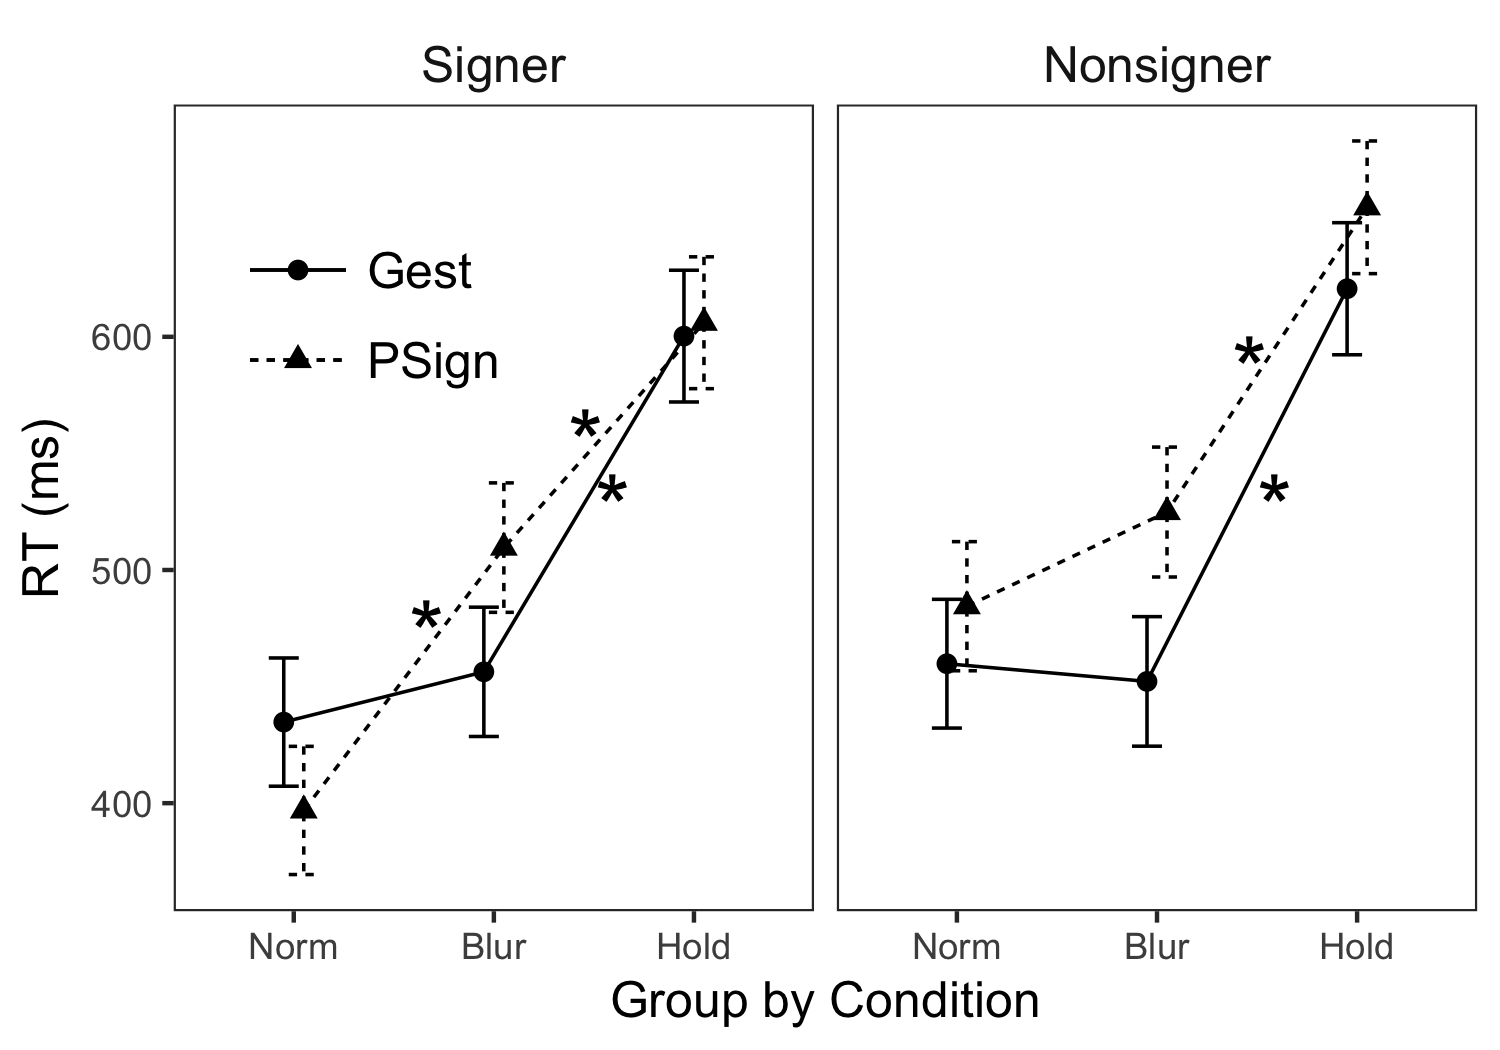
\includegraphics[scale=\sc]{Fig_Trans_Cond} 
                \caption[Parameter estimates: Transitions, effect of Condition]{Parameter estimates for a linear mixed effects model examining the effect of video manipulation Condition and Type on RTs for each group. Gest = Grooming gesture; PSign = pseudosign; Norm = Normal videos.} \label{fig:trans_cond}
            \end{figure} 

            The omnibus test of this model is shown in Table \ref{tab:trans_lme_cond} and parameter estimates for each condition are shown in Figure \ref{fig:trans_cond}. Counter to expectations, and in continuation of a trend from Chapter \ref{ch:shad}, there was no main effect of Group. There was, however, a main effect of Condition, contrasting Normal and Hold, \i{p} $<$ 0.001. This result indicates that participants were using transitional information to generate predictions. Next, the two-way interaction between Group and Type, \i{p} = 0.018, indicates that signers and nonsigners were differentially affected by the Type manipulation. A contrast of marginal linear predictions highlights that, while signers are equally fast for grooming gestures compared to pseudosigns, \chsq(1) = 0.25, \i{p} = 0.62 (\i{M} = 497, \i{SE} = 26.4 vs.  \i{M} = 504,   \i{SE} = 26.4), nonsigners are significantly faster for grooming gestures compared to pseudosign, \chsq(1) = 9.44, \i{p} $<$ 0.01 (\i{M} = 511, \i{SE} = 26.4 vs. \i{M} = 555,   \i{SE} = 26.4).\par
            Planned contrasts for this experiment, however, included an examination of whether each group attended to movement (Blur vs. Hold) or handshape transition (Normal vs. Blur) information in predicting target signs. Contrasts indicated that both signers, \chsq(1) = 120.71, \i{p} $<$ 0.001, and nonsigners, \chsq(1) = 179.2, \i{p} $<$ 0.001, attend to movement information. This is clearly visible in the steep slopes between Blur and Hold conditions in Figure \ref{fig:trans_cond}. Both groups show slower RTs for Hold compared to Blurred videos in both grooming gesture and pseudosign conditions. \par
            An additional planned contrast, looking at handshape transition use in predictions, revealed that signers showed significantly different RTs between Normal and Blurred videos, \chsq(1) = 37.68, \i{p} $<$ 0.01, while nonsigners did not show this difference, \chsq(1) = 2.14, \i{p}  = 0.14. This effect was driven by a     pseudosign stimuli, \chsq(1) = 55.50, \i{p}  $<$ 0.01 (\i{M} = 397, \i{SE} = 27.5 vs. \i{M} = 510, \i{SE} = 27.8). Signers exhibited no such significant difference for grooming gestures, \chsq(1) = 2.04, \i{p}  = 0.15 (\i{M} = 435, \i{SE} = 27.5 vs. \i{M} = 456, \i{SE} = 27.7). While both groups made use of transitional motion information for both stimulus Types, only the signers make use of handshape transitions, and did so only for pseudosigns. Nonsigners did, however, trend in the same direction for pseudosigns (Normal: \i{M} = 484, \i{SE} = 27.7, Blur: \i{M} = 524, \i{SE} = 27.9). A post-hoc test revealed that signers were faster at responding to Normal pseudosign stimuli than nonsigners, \chsq(1) = 5.04, \i{p} = .02 (\i{M} = 397, \i{SE} = 27.5 vs. \i{M} = 484, \i{SE} = 27.7).\par
        \subsubsection{Effect of Symmetricity}
            A very similar model to the one described in the previous section was used to examine the effect of Symmetricity (one- vs. two-handed) items on response times. There are two differences between this model and the previous one: (a) video condition was exchanged for Symmetricity as both a fixed factor and a random slope and (b) this model examines only Normal video response items. The latter decision was made to focus discussion around the nature of predictive representations in a response-to-target setting. Fixed factors in the present model included Symmetricity, Type, Group, and all interactions. Random intercepts include item, item position within the video, and subject, with subject by Type and subject by Symmetricity random slopes. Random intercepts permit variation in overall lag time depending on item or the target’s position within the video. Random slopes permit lag time variation in how each subject exhibits stimuli Type or Symmetricity effects, while still looking at these effects across the dataset. As shown in Table \ref{tab:trans_lme_sym}, these slopes had negligible effects on the model, but were retained to parallel the model shown in Table \ref{tab:shad_lme_sym}.\par

            \begin{table}[!h]\centering \begin{threeparttable}
                \caption[Transitions effect of Symmetricity, mixed effect model]{Summary of effect regressions of RTs across the fixed factors (Symmetricity, stimulus Type and Group), and their interactions.} \label{tab:trans_lme_sym}
                %Table_Trans_LME_Sym.tex
\begin{tabular}{lrrrr} %S[table-comparator = true]}
	\toprule  
	& \multicolumn{1}{c}{Coefficient} & \multicolumn{1}{c}{\i{SE}} & 
	\multicolumn{1}{c}{\i{z}} & \multicolumn{1}{c}{\i{p} $> |$\i{z}$|$}
	\\ \midrule
	\multicolumn{5}{l}{Fixed Effects} \\
	\IE Intercept & 579.935 & 37.922 & 15.29 & $<$ 0.001\\
	\IE Group & -64.272 & 53.512 & -1.20 & 0.230\\
	\IE Sym  & -226.298 & 38.995 & -5.80 & $<$ 0.001\\
	\IE Group * Sym & 68.220 & 54.780 & 1.25 & 0.213\\
	\IE Type & -127.500 & 39.360 & -3.24 & 0.001\\
	\IE Group * Type & 28.568 & 55.262 & 0.52 & 0.605\\
	\IE Sym * Type 		   & 318.268 & 55.505 & 5.73 & $<$ 0.001\\
	\IE Group * Sym * Type & -191.247 & 77.733 & -2.46 & 0.014\\
	\multicolumn{5}{l}{Random Effects} \\
	\IE Subject & & & & \\
	\IE\IE \i{SD} (Intercept) & 14127.97 & 4142.92\tnote{b} &  & \\
	\IE\IE \i{SD} (Type) & 0.086 & \multicolumn{1}{c}{NA\tnote{a}} &  & \\
	\IE\IE \i{SD} (Sym) & <0.001 & \multicolumn{1}{c}{NA\tnote{a}}  &  & \\
	\IE \i{SD} (Item) & 59037.34 & 6312.91\tnote{b} & & \\
	\IE  \i{SD} (Placement) & \multicolumn{2}{c}{NA\tnote{c}}  & & \\
	\bottomrule
	\end{tabular} 
	\begin{tablenotes}
	    \small
	      \item \i{Note}. \i{SD} = Standard Deviation; \i{SE} = Standard Error; \i{p} = p-value significance; Sym = Symmetricity; Placement = Target Placement relative to video. \item[a] As subject slopes contribute minimally to the model, standard deviations are not calculated. These components are preserved in model to parallel Experiment 1 Symmetricity analysis. \item[b] Approximate value provided by nearly identical model, missing subject slopes. All p-values across models remain the same. \item[c] Calculation suppressed due to computational limitations. \end{tablenotes}



	% \multicolumn{5}{l}{Fixed Effects} \\
	% \IE Intercept & 589.913 & 27.091 & 21.78 & 0\\
	% \IE Group & -31.766 & 38.293 & -0.83 & 0.407\\
	% \IE Sym  & -156.598 & 19.158 & -8.17 & 0\\
	% \IE Group * Sym & 37.006 & 26.974 & 1.37 & 0.17\\
	% \IE Type & -39.016 & 19.21 & -2.03 & 0.042\\
	% \IE Group * Type & 4.013 & 27.042 & 0.15 & 0.882\\
	% \IE Sym * Type & 164.094 & 27.257 & 6.02 & 0\\
	% \IE Group * Sym * Type & -82.758 & 38.278 & -2.16 & 0.031\\
	% \multicolumn{5}{l}{Random Effects} \\
	% \IE Subject & & & & \\
	% \IE\IE \i{SD} (Intercept) & 11573.09 & 2818.531 &  & \\
	% \IE\IE \i{SD} (Type) & 0.003 & \multicolumn{1}{c}{NA\tnote{a}} &  & \\
	% \IE\IE \i{SD} (Sym) & < 0.001 & \multicolumn{1}{c}{NA\tnote{a}}  &  & \\
	% \IE \i{SD} (Item) & 14455.24 & \multicolumn{1}{c}{NA\tnote{a}}  &  & \\
	% \IE  \i{SD} (Placement) &  \multicolumn{2}{c}{NA\tnote{b}} & & \\
	% \bottomrule
	% \end{tabular} 
	% \begin{tablenotes}
	%     \small
	%       \item \i{Note}. \i{SD} = Standard Deviation; \i{SE} = Standard Error; \i{p} = p-value significance; Sym = Symmetricity; Placement = Target Placement relative to video. \item[a] As subject slopes contribute minimally to the model, standard deviations are not calculated. These components are preserved in model to parallel Experiment 1 Symmetricity analysis. \item[b] Calculation suppressed due to computational limitations. \end{tablenotes} 
            \end{threeparttable} \end{table}

            \begin{figure}[h] \centering 
                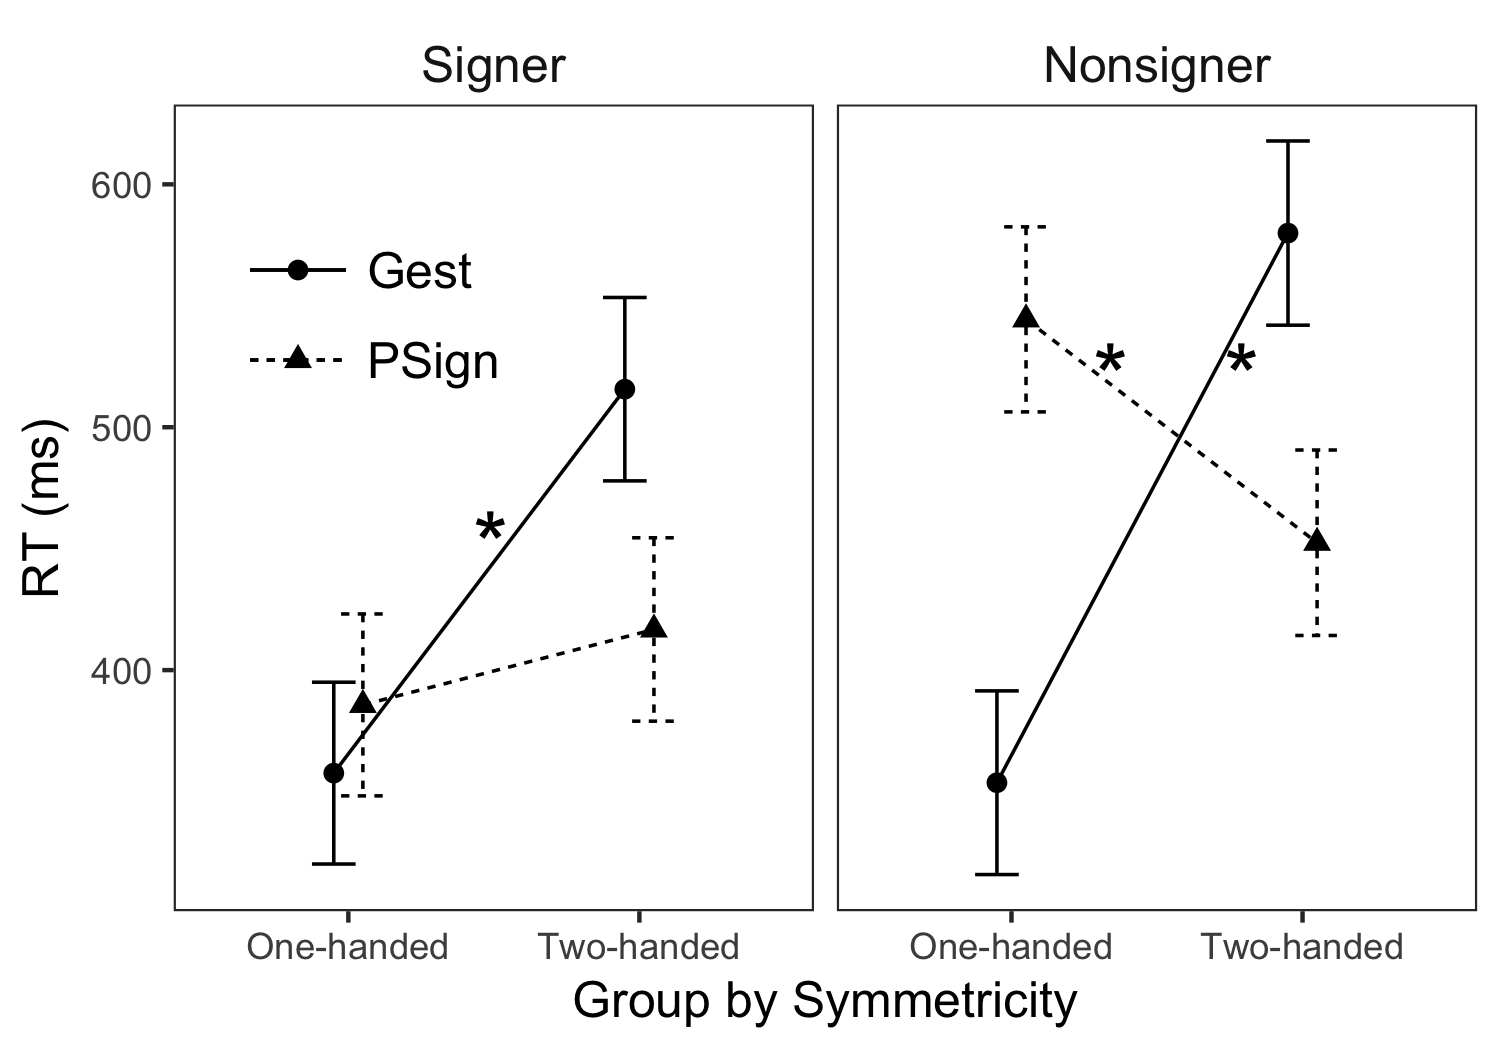
\includegraphics[scale=\sc]{Fig_Trans_Sym}
                \caption[Parameter estimates: Transitions, effect of Symmetricity]{Parameter estimates for a linear mixed effects model examining the effect of Symmetricity and Type on RTs for each group. Gest = Grooming gesture; PSign = pseudosign. \oneS \i{p} $<$ .05} \label{fig:trans_sym}
            \end{figure}

            The omnibus test of this model is shown in Table \ref{tab:trans_lme_sym} and parameter estimates for each condition are shown in Figure \ref{fig:trans_sym}. Consistent with previous models, but counter to predictions, there was no main effect of group. Counter to predictions regarding the difficulty of non-dominant hand suppression, there was a main effect of Symmetricity, \i{p} = 0.001, with one-handed items having faster overall RTs compared to two-handed items (\i{M} = 408, \i{SE} = 22.9 vs. \i{M} = 490, \i{SE} = 23.0). \par
            Finally, this model showed a three-way interaction between Symmetricity, Type and Group, \i{p} = 0.014. Contrasts of marginal linear predictions revealed that both signers, \chsq(1) = 5.45, \i{p} =0.020, and nonsigners, \chsq(1) = 32.88, \i{p} $<$ 0.001, demonstrated an interaction between Symmetricity and Type. Looking at each Group and Type individually, we see that the signers showed Symmetricity effects grooming gestures, \chsq(1) = 16.88, \i{p} $<$ 0.001, but not pseudosigns, \chsq(1) = 0.65, \i{p} = 0.42. Nonsigners showed this effect for both grooming gestures, \chsq(1) = 33.68, \i{p} $<$ 0.001 and pseudosigns, \chsq(1) = 5.42, \i{p} = 0.020, but in opposite directions. For both groups, one-handed grooming gesture response times were faster than two-handed grooming gestures. For the nonsigners, pseudosigns go in the opposite direction: one-handed pseudosigns were significantly slower than two-handed pseudosigns (\i{M} = 544, \i{SE} = 38.1 vs. \i{M} = 452, \i{SE} = 38.2).\par
    \subsection{Discussion}
        %
            The main effect of the video manipulation condition, in the form of large differences between Blur and Hold RTs, is unsurprising. Hold videos give no transition information, such that this condition might as well be a recognition task. Hold is slower in each stimulus type and for both groups. Overall, this indicates that sign experience has no effect on an individual’s ability to instant recognize a target item. While deafness does grant improved ability for certain kinds of visual processing abilities \cite<e.g.,>[]{bosworth2002}, recognition of a target manual production in a rapid-onset video is not one such skill. \par
            Also in line with predictions is the selective effect of Condition (Normal vs. Blur): signers, but not nonsigners, attend to handshape transitions when generating predictions about pseudosigns, but not grooming gestures. This finding points to the notion that sign language experience allows users to attend to intermediate handshapes. It may be the case that signers only attend to intermediate handshapes when sign phonology is present. As discussed on page \pageref{par:hs_complexity}, the pseudosign stimuli involve more marked, and therefore more complex, handshapes. It may be the case that the increased handshape complexity present in the pseudosigns makes the handshape transitions more informative for the signers, or makes for more visually distinct targets for which the signers, but not nonsigners, already have ample motor experience. In any case, this finding aligns with previous research indicating that signers pay attention to intermediate handshapes when comprehending fingerspelling \citeA{cormier2008, brentari1998}. Future research might contrast attention to intermediate handshapes when transitioning between pseudosigns with marked versus unmarked handshapes.
            \par
            The role of symmetricity in this context did not conform to predictions whereby one-handed items would have longer RTs due to non-dominant hand suppression during motor simulation.  The present Experiment was designed with Pickering and Garrod's (2013) proposal in mind. Theoretically, even a button-press task such as this should be accompanied by covert motor imitation to facilitate predictions. This motor simulation was hypothesized to be hindered by the suppression difficulties of one-handed productions. Trends from the present study, however, indicate that one-handed items are easier to predict. This may be grounds for proposing that motoric simulation is not fully active during a response-to-target task. It may be the case that attending to two hands in this task is more cognitively demanding (i.e., attending to two articulators rather than one), and is therefore a slower process. Because nonsigners only demonstrated the symmetricity effect for grooming gestures, it may be the case that this increased cognitive demand of attending to two hands was continued when nonsigners viewed one-handed pseudosigns. \par
            Taken together, these results indicate, first, that transitional movement plays a major role in the predictive representations used to identify the target in this context. This holds true for both groups in both linguistic and nonlinguistic contexts. Second, signers were uniquely capable of using handshape transition information to generate predictive representations. This finding supports the notion that sign language experience supports a user’s ability to attend to transitional handshape information, as discussed in \citeA{cormier2008} and \citeA{geer2017}. Counter to expectations, this ability among the signers did not extend to a nonlinguistic context. Handshape-based predictive representations may be domain-specific. Or, it may be the case that handshape transitions are only useful in high handshape complexity contexts (i.e., pseudosign). Third, as one-handed predictions were, in general, faster, the present results run counter to the notion that all predictive representations are motoric. It may be the case that motor representations are subtle in button-push tasks, or that, as a push-button task, actively using one’s dominant hand may suppress any motor representations participants would have ordinarily used in such a passive task. Finally, it may be that non-dominant hand suppression only plays a role during overt production and does not interfere with covert imitation. \par
            While this Experiment cannot support strong proposals of ever-present motor simulation for both linguistic and nonlinguistic predictions, it does provide insight into how sign language experience shapes phonological representations of transitional information. In particular, both signers and nonsigners are using movement information to generate predictions, but sign language users were unique in employing handshape transitions in linguistic predictive representations. This finding aligns with previous reports regarding the utility of transitional information for signers, but not nonsigners \cite{geer2014}. The Experiment to follow will look for evidence that these groups differ in offline motor simulation abilities, outside of predictive contexts\footnote{This chapter, in part, is currently being prepared for submission for publication of the material. Brozdowski, Chris; Emmorey, Karen. The dissertation author was the primary investigator and author of these materials.}. 

\section{Experiment 3: In Support of Forward Models, Simulation and Memory}  
    \label{ch:supp} 
    \subsection{Introduction} \label{sec:supp_intro}
        %%
            Covert imitation is a key component of Pickering and Garrod 's (2013) proposal on forward modeling. While Pickering and Garrod don't go into substantial detail about the specifics of other processes that may support covert imitation, the imitation itself is described as motoric simulation. Experiment 1 measured covert imitation of a model by asking participants to make their covert imitations overt; shadowing tasks participants with generating and acting out predictive representations. Experiment 2 measured predictive representations of a model, in part, by examining how informative early transitional cues can be to responding to a stimulus. The one- vs. two-handed item comparison was able to draw conclusions about the degree to which motoric simulation facilitates response-to-target predictive representations. These time-sensitive, or ‘online’ tasks directly measured predictive abilities as predictions were being made. In contrast, offline tasks can provide more insight into the mechanics of predictive processing by examining related abilities. \par 
            The first of two tasks in the present Experiment, the Test of Ability in Movement Imagery for hands, examines motoric simulation of one’s own body in a non-predictive, offline task. The second task, Motor Memory (MM), separates viewing action from providing a response, and measures storage of movements rather than active simulation. As such, this task represents a measure of motoric maintenance and execution. The following Chapter will examine to what extent tasks from Experiments 1 and 2 can be associated with offline motor simulation and motor memory by looking at correlations between these measures. The present Chapter, however, will focus strictly on performance on each of these offline measures individually.  Sign language experience was expected to grant users both improved ability to imagine complex handshapes as well as greater ability to efficiently encode motoric information for retrieval. Signers were, therefore, predicted to show improved ability for both tasks relative to nonsigners. 
            \citeA{donoff2018} developed the Test of Ability in Movement Imagery for hands (TAMI-h). This test is a hand-specific version of the TAMI, a full-body measure developed by the same group \cite{madan2013}. In each case, participants are given a booklet of multiple-choice questions. Each question is presented as a set of instructions for how to position oneself. The first instruction asks participants to imagine their hand or body in a neural position. Four subsequent instructions then manipulate this imagined neutral position by changing the position of one or more fingers or limbs. Taking the TAMI-h, one would start by imagining one’s hand in a flat B handshape before manipulating this neutral position with subsequent written instructions, such as "touch the tip of your thumb midway up your ring finger." The original TAMI has similar instructions sequentially applied to the full body, instructing the participant to “Step your left foot forward 30 cm,” for example. During the TAMI-h, the participant is prevented from executing instructed movements by holding a tennis ball in the relevant hand. The ball serves to ensure that all motor movements are imagined.  Actually positioning one’s hand is a very effective strategy, but wouldn’t engage the simulation abilities desired. \par
            Once the participant has imagined a handshape, they must select either from a set of hands or a set of objects. For example response sets, see Section \ref{sec:tami_example} of the Appendix. None of the handshapes imagined in this test are exact matches to those found in the ASL inventory of handshapes, and are thus considered to be nonlinguistic. Response sets of pictures are part of the Isolated imagery subtest, directed at only testing an individual's ability to imagine hands out of context. The object images are part of the Functional imagery subtest, directed at assessing an individual's ability to imagine object-oriented handshapes. In addition to the predicted relationship between sign language experience and overall TAMI-h performance, it was further predicted that signer benefits would be tied more to the Isolated than the Functional conditions. \par
            While signers undoubtedly have greater experience perceiving and executing linguistic contrastive handshapes, generalized motor imagery has not yet been studied in this group. One possibility is that sign language experience is tied to drawing distinctions between contrastive handshapes: detailed fine-motor representations are unimportant so long as one can faithfully recognize and execute linguistic handshapes. On the other theoretical hand, and from the perspective of motor simulation proposals \cite<i.e.,>[]{PG}, sign language experience rehearses covert motor imitation of not only target handshapes, but transitional handshapes that do not conform to typical linguistic distinctions \cite{schwarz2000, geer2017}. Just as sign language perceptual expertise for transitional information was hypothesized to transfer to nonlinguistic contexts in Experiments 1 and 2, signer linguistic imagery abilities were hypothesized to transfer to nonlinguistic contexts. Signers were, therefore, predicted to have better ability to imagine complex handshapes independent any object-oriented action due to their greater experience imagining complex handshapes in linguistic contexts. \par
            The Functional subtest of this measure served as an opportunity to examine how generalizable this knowledge may be. Sign language sometimes employs handling handshapes that simulate the use of an object \cite{sandler2006}. While it is possible that such sign language experience would transfer to an offline test of object-oriented motor imagery, these handling handshapes are relatively infrequent and were not hypothesized to bolster motor imagery in the present context. Signers and nonsigners were expected to perform similarly for Functional questions. \par
            Prior work with the TAMI-h focused on handedness effects as well as contextualizing this task within broader handedness and imagery work \cite{donoff2018}. In brief, participants performed better when the version of the task matched their own hand dominance: right-handed participants scored higher on the right-handed version of this task. There was a handedness by subtest interaction: hand dominance showed a greater impact on scores for Functional, compared to Isolated, questions. In other words, imagined isolated movements may be more generalizable across both hands and may engage a more generalizable kind of imagery, while experience with functional handshapes may be more tied to an individual’s specific experiences. Rather than being tied to abstract imagery, for example, previous findings would suggest that individual variation on the Function subtest is tied to experience using those specific objects (e.g., hammer, computer mouse, etc) and not sign language experience. \par
            \citeA{donoff2018} also examined performance on TAMI-h without and without instructions designed to promote an egocentric frame of reference for the task. In absence of any difference between these conditions, \citeA{donoff2018} concluded that participants naturally apply an egocentric frame of reference to the task. In other words, participants naturally complete the task by imagining themselves executing the motor instructions provided. All predictive processing, according to the Pickering and Garrod (2013) model, should engage similar covert egocentric motoric simulation. Increased experience or expertise in manual motor simulation among sign language users was expected to lead to increased signer performance on this task relative to nonsigners. \par
            Pickering and Garrod’s (2013) model deals directly with motor stimulation and representations about the immediate future, and, as presented, is not necessarily associated with to other abilities. This model of language comprehension allows an underspecified ‘contextual information’ module to play a role in covert imitation. More recent evidence by \citeA{huettig2016} describes working memory as a mediating factor in predictive language abilities and presents evidence to that effect. More specifically , \citeA{huettig2016} presented participants with Dutch sentences such as “look at the presented piano,” with either the common- or neuter-gendered article. Participants were visually presented with objects that could be referred to with either gender article. In general, participants demonstrated predictions about the noun to follow via proportional eye gaze to the relevant article-matching pictures. \citeA{huettig2016} then compared individual variation on this predictive language measure to measures of processing speed \cite<digit-symbol substitution;>[]{ wechsler2014}, as well as both auditory \cite<non-word repetition;>[]{wechsler2014} and spatial memory \cite<Corsi block test;>[]{corsi1972}. \par
            \citeA{huettig2016} make the case that their predictive language measure is independently related to both processing speed and working memory.  In the context of their eyetracking task, participants’ (a) ability to rapidly process the auditory language, and (b) visual memory of the object presented on the screen both likely facilitated predictive representations of the incoming sentence. In the context of Shadowing and predictive response-to-target task, as presented in Chapters \ref{ch:shad} and \ref{ch:trans}, predictive representations of incoming stimuli may be related to participants’ ability to retain a lexicon of the possible items. The present Chapter will examine whether or not groups differ in their motor short-term memory capacities and whether or not these memory capacities differ for grooming gesture versus pseudosign. It was predicted that experience with sign language phonology would result in improved ability retain pseudosigns. \par
            The novel short-term Motor Memory (MM) task presented here was based on Wu and Coulson's \citeyear{wu2014} body movement working memory test. \citeA{wu2014} presented participants with verbal working memory (sentence span) and spatial working memory \cite<Corsi block;>[]{corsi1972} tasks, in addition to a novel motor memory measure. Their novel task asked participants to watch and repeat meaningless movements, primarily articulated on the arms. At first, only one movement was presented for each of three trials. If a participant could accurately recall (i.e., get at least half credit) for these three trials, the participant would move on to seeing three trials of two movements each. Span level, or span length, refers to the number of movements in a given trial. Half credit was awarded to any production that reflected a memory of the movement with imperfect production. Cumulative score refers to the accumulated number of points a participant received before the test was discontinued due to poor performance. \citeA{wu2014} found no correlation between their span length or cumulative scores on their verbal or spatial working memory tasks, drawing conclusions about the relative independence of motor, verbal and spatial working memory abilities. 
            The tasks presented in Experiments 1 and 2 both assess motoric simulation and prediction of grooming gestures and pseudosigns. While the the specific stimuli from \citeA{wu2014} were well-targeted to memory for novel motor movements, Experiment 4 of the present work was designed to examine the relationship between linguistic and nonlinguistic processing, and thus required a task with well-matched items along these lines. Stimuli from \citeA{wu2014} were found to be multi-syllabic in a way that (a) did not map well onto ASL phonology and (b) was more complex than typical pseudosigns. Stimuli presented in Experiments 1 and 2 (see Table \ref{tab:stim} on page \pageref{tab:stim}), however, already match in general complexity across subtests, and were used for the present Motor Memory task. While both nonlinguistic, grooming gestures in the present works are both simpler and more familiar to participants than the meaningless movements presented by \citeA{wu2014}. As such, results from the two tasks will not be directly comparable. The MM task, as a result of reduced complexity of individual items, was also extended to include additional span levels (up to seven) not included in \citeA{wu2014}. \par
            Concerning how memory and motor simulation abilities may differ across groups, sign language experience was expected to give users more efficient storage abilities for pseudosigns. Signers were therefore predicted to perform better on this subtest than the grooming gesture equivalent. Following Wu and Coulson’s (2014) proposal that motor memory is separate from other forms of working memory, it was hypothesized that sign language experience would train motor memory abilities across domains. Signers were predicted to outperform nonsigners on this task. \par
    \subsection{Methods} \label{sec:supp_meth}
        \subsubsection{Participants}
            Those participants recruited for Experiment 2 also completed the TAMI-h immediately after the Transitions task. While the Transitions scores for twelve nonsigner participants were excluded due to technical error, TAMI-h scores from these participants were still useful for examining performance on this task in isolation. Altogether, 21 Deaf signers (13 Female, \i{M} age = 35.50, \i{SD} = 9.78) and 32 sign-na\"ive English speakers (21 Female, \i{M} age = 33.61, \i{SD} = 14.81) completed the TAMI-h. All participants were right handed. \par
            Those recruited for Experiment 1 also completed the Motor Memory (MM) task immediately after the Shadowing task. This includes the one participant who failed to shadow in the former task, but excludes one participant for whom there were technical difficulties with the WM task. Altogether, 20 Deaf signers (12 Female, \i{M} age = 37.01, \i{SD} = 10.55) and 19 sign-na\"ive English speakers (14 Female, \i{M} age = 39.72, \i{SD} = 16.99) completed the MM task. \par
        \subsubsection{Materials/Procedure}
            The TAMI-h was designed by \citeA{donoff2018} and includes four distinct versions: two to assess left hand imagery and two to assess right hand imagery. Here, TAMI-h scores reflect only the right-hand versions, counterbalanced across participants. After completing the Transitions task from Chapter \ref{ch:trans}, participants sat at a table and were given a packet, pen, answer sheet and tennis ball. Participants were instructed to (a) read the instruction sheet and each of the questions carefully, (b) imagine the handshape described by sequential instructions for each trial, (c) turn the page and do not look back to the questions and (d) hold the tennis ball in the right hand firmly while both reading and selecting a response. The tennis ball, when correctly held, requires muscle tension to hold and is designed to suppress overt muscular activation. Participants were told to only put down the tennis ball after they had decided the correct answer and to place the ball on the table in order to write the appropriate letter on their answer sheet. Approximately half of the trials were accompanied by a set of pictures of hands, targeting Isolated hand imagery, and half of the trials were accompanied by a set of pictures of objects, targeting Functional hand imagery. \par
            For Isolated trials, there was one correct picture, yielding one point. For Functional trials, each of the possible response pictures was associated with a point value: two, one, half or zero points were given depending on the response. Scores were calculated as a percent of possible points for a given subtest, as each of the two versions administered have different possible point values for the subtests. Where reported, a general TAMI-h score reflects an average of the two subtests. \par
            \citeA{wu2014} designed their kinesthetic WM test to include complex multi-part arbitrary movements. The present MM test replaces these movements with the pseudosign and grooming gesture items as shown in \ref{tab:stim} on page \pageref{tab:stim}, and includes a one second inter-stimulus interval, in accordance with short-term memory span paradigms for words and signs \cite{hall2011}. This task preserves all coding scheme and span test design features from Wu and Coulson’s (2014) test, but the task extends the maximum span from five to seven and includes a Subtest for each stimulus type. For each trial, the MM task presents participants with one or more items (pseudosign or grooming gesture) inventories. After each trial, participants were instructed produce the movements shown in the videos in the order they were presented. At the first level (i.e., span length), each trial consists of one stimulus; at the second level, each trial consisted of two stimuli, and so forth. There are seven total levels. After each item is presented, the final frame is held for a one second inter-stimulus interval. Lists are balanced to include equal numbers of each possible item. \par
            Cumulative score for this task was measured by assigning one point for each correctly reproduced item and calculating the sum. For any given stimulus, a participant receives one point for a correct production and zero points for an incorrect production. Half credit is awarded for productions with one phonological parameter deviating from the target, demonstrating some memory of an item with a flawed production (e.g., correct movement and location but an incorrect handshape). No credit is awarded for a given item if (a) the participant displays no recollection of the item and/or produces a different item, or (b) only demonstrates recollection of one phonological parameter (e.g., hands move near face to indicate ‘the sign location was somewhere in this location’). A participant is permitted to move to the next level (i.e., span length) of the test if they received at least half of all possible points for a given level. As discussed on page \pageref{par:hs_complexity}, grooming gesture and pseudosign items were matched for item location, but differ in handshape complexity. The pseudo-randomized order of item presentation was preserved across subtests: if a given trial for the pseudosigns presented participants with item numbers 1, 7, 4 and 10, for example, this was paralleled by a trial with the name numbered location-matched grooming gestures. Subtest order was counterbalanced across participants. \par
\subsubsection{Analysis}
            A 2x2, Group by Subtest, mixed repeated measures ANOVA, with Group as a between-subject factor, was conducted for each task. For TAMI-h, the subtests are Isolated and Functional. For the MM task, subtests are each of the stimulus types, grooming gesture and pseudosign. Post-hoc paired t-tests were used to follow-up on trends revealed by ANOVAs.\par
    \subsection{Results}
        %
            The ANOVA of TAMI-h percent accuracy scores showed a marginal effect of Subtest, \i{F}(1,51) = 3.251, \i{p} = .077. Participants had marginally higher scores for Isolated (\i{M} = 63\%, \i{SD} = 27\%) compared to Functional items (\i{M} = 57\%, \i{SD} = 16\%). This trend aligns with a significant difference found in \citeA{donoff2018}, even though percent scores are slightly lower than those found in the previous work (Isolated: \i{M} = 76\%, \i{SD} = 1.9\% vs. Functional: (\i{M} = 59\%, \i{SD} = 2.1\%). There was neither a main effect of Group, \i{F}(1,51) = 0.151, \i{p} = 0.70, nor an interaction between Group and Subtest, \i{F}(1,51) = 0.281, \i{p} = 0.60. Means for this task are shown in Figure \ref{fig:tami}.\par

            \begin{figure}[!h] \centering
                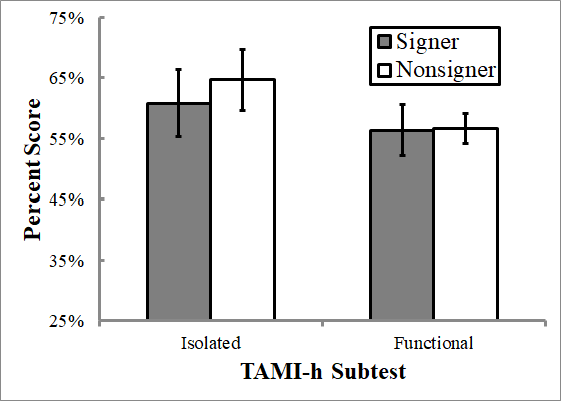
\includegraphics[scale=.8]{Fig_TAMI} 
 
                \caption[TAMI-h means by Group and Subtest]{Percent performance (mean and standard error) on the hand Test of Ability in Movement Imagery by Group and Subtest. Isolated items match imagined hands with pictures of hands, while Functional items match imagined hands with manipulable objects.} \label{fig:tami} \end{figure} 

 
            
            The mixed ANOVA of MM cumulative scores shows a similar marginal effect of of Subtest, \i{F}(1,37)=3.48, \i{p} = .070, with participants, on average, showing higher cumulative scores for the pseudosign (\i{M} = 36, \i{SD} = 16) compared to grooming gesture Subtest (\i{M} = 32, \i{SD} = 11). There is neither a main effect of Group, \i{F}(1,37)=1.00, \i{p} = .324, nor an interaction, \i{F}(1,37)=1.76, \i{p} = .198. Post-hoc paired t-tests reveal, however, that signers showed a significantly higher performance for pseudosigns compared to grooming gestures, \i{t}(19) = -3.456, \i{p} =.003, while nonsigners showed no such difference, \i{t}(18) = -.308, \i{p} =.762. Mean cumulative scores for each Group and Subtest are shown in Figure \ref{fig:wm}. \par

 

            \begin{figure}[!h] \centering 
                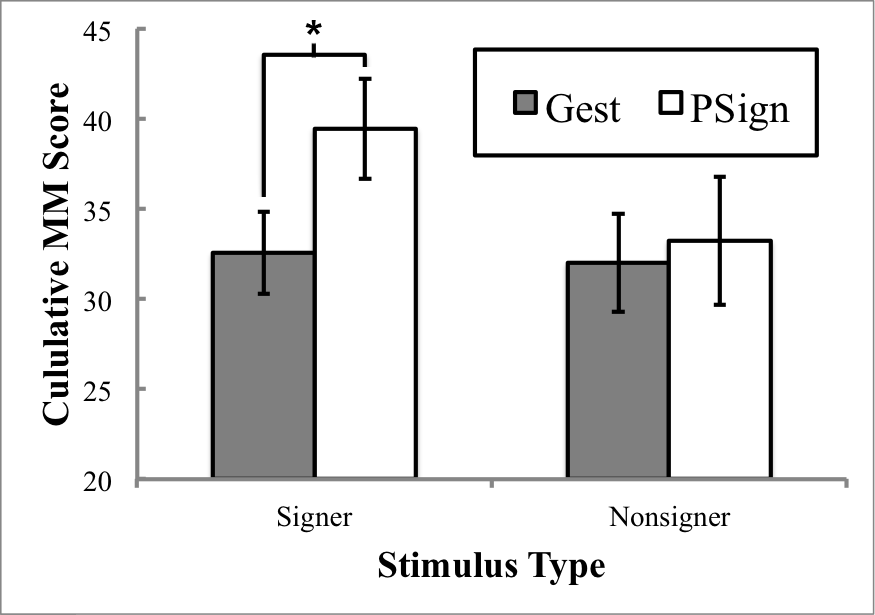
\includegraphics[scale=.8]{Fig_WM} 
 
                \caption[Working memory cumulative scores by Group and Subtest]{Cumulative scores and standard errors on the Working Memory test, by Group and Action Type, grooming gesture (Gest) or pseudosign (PSign). \oneS \i{p} $<$ .05.} \label{fig:wm}
            \end{figure} 
    \subsection{Discussion}
        %   
            This Experiment was designed to look at abilities that may support the predictive representations directly assessed in Experiments 1 and 2. The TAMI-h was chosen to capture an offline measure of egocentric motor simulation. Looking at this test alone, the marginally higher scores for Isolated compared to Function items parallels the significant difference found by \citeA{donoff2018}. The lack of significant finding in the present case is likely a power issue: while \citeA{donoff2018} had 79 participants complete the task, the present study reflects approximately 20 subjects in each group. Regarding group differences, it was hypothesized that experience with motor simulation in sign language use would be associated with improved motor imagery abilities outside linguistic contexts. Counter to expectations, signers and nonsigners show equivalent scores on this hand-specific imagined motor movement task. It may be the case that any relationship between sign language experience and imagined motor movement is domain specific and does not transfer to handshapes not found in ASL’s phonological inventory (see Section \ref{sec:tami_example} for an example). A future version of this test might target phonologically permissible handshapes to further examine the relationship between sign language experience and motor imagery. \par
            One potential limitation of TAMI-h in the present context is the degree to which it relies on reading ability via complex instructions such as "Point your index and middle fingers 45° to the plane of your palm.” While the present work was not designed with a focus of reading ability, concurrent projects have collected reading measures for a subset of the participants in this study. Specifically, eight of the nonsigners and all twenty-one signers took the reading comprehension subtest of the Peabody Individual Achievement Test (PIAT) \cite{PIAT}. Both groups show a relationship between average TAMI-h scores and PIAT reading comprehension. For signers, this is a significant correlation, \i{r}(20)=.497, \i{p}= 0.026, but the correlation is marginal for the relatively few nonsigners who took both tasks, \i{r}(7)=.689, \i{p}= 0.087. There is also a significant difference between groups on PIAT comprehension scores, \i{t}(37) = -2.24, \i{p} = 0.033.  Future research could either address this issue by recruiting groups matched for reading ability or by ensuring that all participants have available reading scores in order to include reading ability as a covariate in analyses. \par
            The Motor Memory test parallels the findings from the TAMI-h. First, signers and nonsigner show equivalent overall memory abilities; sign language experience does not grant overall improvements to motoric memory. Instead, these benefits seem to be limited to the pseudosign performance, with signers performing better on the pseudosign subtest than the grooming gesture and nonsigners performing equivalently across these two stimulus types. The dissociation between signers’ subtest scores reinforced the notion that signers maintain such information in a phonological loop \cite{wilson1997, hall2010}. Although the pseudosign subtest can be comfortably labeled as a non-word span task for the signers, the grooming gesture subtest is more difficult to categorize. Grooming gestures do not conform phonological rules, but are both familiar and functional. The closest vocal equivalent might be a recall task for many unique ways to clear one’s throat, as a self-directed adjustment.  Equivalent grooming gesture scores for signers and nonsigners indicates that the benefits associated with sign language experience do not generalize to nonlinguistic contexts in virtue of shared articulators. \par
            Again, in parallel with the TAMI-h, there is an additional factor to consider for this working memory measure: the current coding system, while typical of memory measures, only noted accuracy and doesn't distinguish between gross phonological and serial position errors. An incorrectly produced target item (i.e., two incorrect parameters wrong) and a misremembered non-target item are both awarded zero points. In designing the coding system, no effort was taken to note if an item was omitted or swapped with another item in the order. The only coded variable was accuracy at the appropriate serial position. The dependent variable, cumulative score, would not capture, for example, if nonsigners produced more phonological errors, but signers had more difficulty with the order. Such a pattern would align with previous proposals that signers have greater difficulty with serial position \cite<e.g.,>[]{bavelier2008}, or might simply reflect different encoding strategies across groups. More recent evidence points to English being a more efficient for encoding in similar span tasks \cite{hall2011, emm2017}. The only existing measure comparing phonological errors across groups is the number of half-credit responses (i.e. one, but not two parameters different from the target item), but groups show no significant differences. In sum, while the present test did little to control language encoding strategies across deaf signers and hearing nonsigners, future analyses on this dataset might re-score videos for number of serial position errors versus number of phonology errors to see if signer and nonsigner groups differ in these error types\footnote{This chapter, in part, is currently being prepared for submission for publication of the material. Brozdowski, Chris; Emmorey, Karen. The dissertation author was the primary investigator and author of these materials.}.  \par

\section{Experiment 4: The relationship between prediction ability, motor memory, and motor memory} 
    \label{ch:correl}
    \subsection{Introduction}
        %
            Although \citeA{PG} discuss forward models in terms of immediate predictive representations, there is little work regarding to what extent these representations are facilitated by related abilities. Section \ref{sec:supp_intro} discusses the theoretical link between covert imitation, as proposed by Pickering and Garrod (2013), and offline motor imagery, as well as existing evidence linking predictive syntactic processing with auditory and spatial working memory abilities \cite{huettig2016}. \par
            The following correlative analyses focus, first, on demonstrating overlap between predictive abilities across the Shadowing and Transitions tasks from Experiments 1 and 2. In theory, both tasks are rooted in motoric simulations that give rise to forward models. In practice, Shadowing entails much more active motoric engagement, and the response-to-target methodology from Experiment 2 is much more susceptible to visual strategies. Different patterns of results regarding the effect of Symmetricity across these two Experiments demonstrate clear differences between the two tasks. Scores from these two tasks were nevertheless predicted to correlate with each other to the extent that both entail close monitoring of the immediate future. \par
            Second, the present Experiment examines to what extent these two predictive tasks rely on the motor memory or hand imagery abilities, as assessed in Experiment 3. To what extent does each contribute to predictive representations? \citeA{huettig2016} discuss their demonstrated relationship in terms of an individual’s ability to maintain visuo-spatial information about the possible outcomes. Similarly, participants’ Experiment 1 Shadowing abilities may be supported by better motor memory for the full inventory of possible items. Because Shadowing may depend on motor memory for an ad hoc lexicon of grooming gestures and pseudosigns, Shadowing was expected to significantly correlate with the Motor Memory task.\par
            Motor memory was hypothesized to also play a similar role in accessing the ad hoc lexicon of experimental items during the Transitions task. Memory was further predicted to play a role in this response-to-target task because it directly entails maintaining a target in memory while generating predictive representations. Additionally, motor memory was expected to play a greater role when predictive processing was least useful, in absence of transitional information. As such, Hold videos were expected to show a stronger correlation with the Motor Memory task. In the Normal condition, responses can be facilitated by more detailed motor representations of motion and trajectory. The Hold condition, by contrast, can be performed by a visual match between the remembered target and video onset. This, as an effective strategy, would make Hold performance more memory dependent. The transitional held frame in this condition, the final frame of the previous item, might also serve to inhibit the appropriate motor representation for the target by instead fixating on the motor execution of the previous item. \par
            In the original paper, \citeA{donoff2018} presented the TAMI-h with and without instructions designed to promote egocentric strategies (i.e., imagining one’s own hand when in various positions in order to complete the task), and concluded that all participants, regardless of instructions, defaulted to this strategy. Although the TAMI-h is an offline measure, such an egocentric motor simulation strategy is a close parallel to motor stimulations as described by Pickering and Garrod (2013). In the context of the Experiment 2, it was hypothesized that participants would generate motor simulations of observed pseudosigns and gestures. Here, it is hypothesized that the TAMI-h taps into similar resources, and a correlation was expected between TAMI-h percent scores and overall Transition response times. Of the TAMI-h subtests, Isolated and Functional, both engage motoric simulation abilities, but the Isolated subtest is more akin to Transitions motor simulation insofar as both are object independent, and was therefore predicted to show a stronger correlation with Transitions response times than the Functional subtest. \par 
    \subsection{Methods}
        \subsubsection{Participants}
            Shadowing and MM scores were available for 39 right-handed participants: 20 Deaf signers (12 Female, \i{M} age = 37.0, \i{SD} = 10.6), and 19 sign-na\"ive English speakers (15 Female, \i{M} age = 38.8 \i{SD} = 17.4). Of the 39, eighteen (16 signers, 10 Female, \i{M} age = 34.4, \i{SD} = 10.0) were able to participate in all tasks: Shadowing, Transitions, TAMI-h and MM. \par
        \subsubsection{Materials/Procedure}
            For details on materials and procedure of specific tasks, see relevant Methods descriptions from various Experiments, Sections \ref{sec:shad_meth}, \ref{sec:trans_meth}, and \ref{sec:supp_meth}. In brief, for the Shadowing task, participants followed along with manual stimuli, generating productions in tandem with various models, which allowed a direct measure of their imitation abilities, as a proxy for the covert imitation described in Pickering and Garrod’s (2013) forward modeling proposal. These same participants then watched videos of increasing length and repeated observed actions in the same order, to test motor memory abilities. Eighteen participants returned on a separate day to participate in the response-to-target task (i.e., Transitions). Participants were shown an image of a gesture or pseudosign and asked to press a button as soon as they identified this item in the context of a longer video. See Table \ref{tab:stim} on page \pageref{tab:stim}, for list of possible items. One third of videos showed the model as filmed (Normal), one third blurred the hands during transition periods between actions (Blur), and one third held the final frame of the action until the onset of the subsequent action (Hold). The final condition showed no transition information whatsoever. Among conditions, Hold videos allowed for the least amount of predictive processing, and my have inhibited motor stimulation for the target item by presenting the final frame of an alternative item until the exact moment of target onset. These participants then completed the TAMI-h \cite{donoff2018}. \par
            Scores for various tests were averaged across subtests: for Shadowing, Transitions, and MM tasks, scores were averaged across the pseudosign and grooming gesture conditions. Unless otherwise specified, Shadowing and Transitions scores were averaged across experimental condition, model and video condition respectively. Bivariate Pearson correlations were performed on subsets of the following variables: average Shadowing lag time, average Transitions RT, Transitions Normal RT, Transitions Hold RT, MM cumulative score, TAMI-h average percent score, TAMI-h Isolated percent score, and TAMI-h Functional percent score. MM scores reflect total accumulated points, rather than span (i.e, maximum list length). All reported significant correlations with MM scores were also significant for MM span, except for one case of marginal significance, \i{p} = .056. For the TAMI-h, Isolated items paired descriptions of complex handshapes with pictures of hands. Functional items paired handshapes with objects that hand might manipulate. For examples, see Figure \ref{fig:tami_example} within the Appendix. Where appropriate, some analyses look to see if a significant correlation is driven by a specific subtest. \par
    \subsection{Results}
        %
            First, a correlation between mean Shadowing lag times and mean response-to-target RTs from Transitions indicated that these two tasks tap into similar predictive processes, \i{r}(18) = .586, \i{p} = 0.011. Broken down by Transitions condition, mean shadowing times significantly correlated with Normal Transitions videos, \i{r}(18) = .608, \i{p} = 0.007, but showed a marginal relationship with Hold videos, \i{r}(18) = .452, \i{p} = 0.055. \par
            Second, a correlation between mean Shadowing lag times and MM cumulative score was performed for each group. While signers showed no relationship between these measures, \i{r}(20) = -.065, \i{p} = 0.786, nonsigners do seem to rely on motor memory abilities in order to complete the Shadowing task, \i{r}(18) = -.541, \i{p} = 0.020. \par
            A similar pattern was observed when looking at the relationship between mean Transitions RTs and TAMI-h percentage scores. While signers showed no relationship between handshape imagery abilities and the response-to-target predictive task, \i{r}(21) = -.021, \i{p} = 0.928, nonsigners showed a significant relationship between scores, \i{r}(21) = -.529. \i{p} = 0.014. In accordance with predictions, further examination revealed that this correlation was driven by this Isolated subtest, \i{r}(21) = -.607, \i{p} = 0.004. Nonsigner Transitions RTs show no relationship to the Function subtest of the TAMI-h, \i{r}(21) = -.094, \i{p} = 0.684. \par
            Forth, there was a significant relationship between mean Transitions RTs and cumulative MM scores for the 16 signers and 2 nonsigners who completed both tasks. There was an overall relationship between Transitions RTs and MM cumulative scores, \i{r}(18) = -0.500, \i{p} = 0.035, but this was driven by the Hold items from the Transitions experiment, \i{r}(18) = -0.524, \i{p} = 0.026. There was no significant correlation between Transitions and Normal items, \i{r}(18) = -0.331, \i{p} = 0.179.

            \begin{table}[!h]\centering \begin{threeparttable} 
            \caption[Inter-experimental correlation coefficients]{Bivariate correlation coefficients between major tasks in the present work, broken down by language group: Shadowing (Shad), Transitions (Trans), both Normal (TNorm) and Hold (THold) Conditions, Motor Memory (MM), and TAMI-h, both Isolated and Functional Subtests.} \label{tab:correl}
            %Table_correl.tex

% Bivariate correlation coefficients between major tasks in the present work, broken down by language group: Shadowing (Shad), Transitions (Trans), both Normal (TNorm) and Hold (THold)Conditions, Motor Memory (MM), and TAMI-h, both Isolated and Functional Subtests.

\begin{tabular}{lcccc}
    \toprule  
    Measure  & \multicolumn{1}{c}{Shad} & \multicolumn{1}{c}{Trans} & \multicolumn{1}{c}{TNorm} & \multicolumn{1}{c}{THold}  \\ \midrule 
    \multicolumn{1}{l}{Both Groups} &  &  &  &   \\
    \IE Shad & --- &  &  &   \\
    \IE Trans & .586\oneS & --- &  &   \\
    \IE \IE TNorm & .608\twoS &  & --- &   \\
    \IE \IE THold & .452\marS &  &  & ---  \\
    \IE MM &  & -0.500\oneS & -.331\nonS & -.524\oneS  \\
    Signers &  &  &  &   \\
    \IE MM & -.065\nonS &  &  &   \\
    \IE TAMI-h &  & -.021\nonS &  &   \\
    Nonsigners &  &  &  &   \\
    \IE MM & -.541\oneS &  &  &   \\
    \IE TAMI-h &  & -.529\oneS &  &   \\
    \IE \IE Isolated &  & -.607\twoS &  &   \\
    \IE \IE Functional &  & -.094\nonS &  &   \\
    \bottomrule \end{tabular} \begin{tablenotes}
    \small
      \item \i{Note}. \nonS \i{p} $>$ .1, \marS \i{p} $<$ .1, \oneS \i{p} $<$ .05, \twoS \i{p} $<$ .01. \end{tablenotes}


            \end{threeparttable} \end{table}

 

\subsection{Discussion}
        %
            The significant correlation presented between Shadowing and Transitions serves as confirmation that both tasks require predictive motor processing. The relationship between these two tasks supports Pickering and Garrod’s (2013) general notion that motoric predictive representations active during passive comprehension. The Shadowing task forces participants to be explicit about their motor representation; it forces covert imitations to become overt. While more passive, the Transitions task can still be understood as predictive in light of the penalties incurred when removing transitional information. Even when no predictive processing is required for Transitions, in the case of the Hold videos, there is still a marginal relationship with mean Shadowing lag times. This could be interpreted as either (a) an indication that predictive processing is engaged even when no transitional information is available or (b) an indication that both tasks require more resources than predictive processing alone. Additional resources might include non-predictive body motion processing ability, for example. Future research might attempt to disentangle these two explanations by examining response-to-target abilities for inanimate stimuli. \par
            The response-to-target Transitions task differs from Shadowing in the requirement that one maintain some representation of the target between target presentation prior to the video and target onset in the context of the video. It is unsurprising, then, that mean Transition reaction times correlate with overall motoric memory abilities. First, this correlation affirms that the memory task is indeed assessing maintenance of motoric information. The Transitions Hold videos could be described as sequential presentations of various stimuli with variable inter-stimulus intervals related to the length of transitions. The presence of an alternative image prior to target onset may even inhibit the correct motor simulation, but the only fair comparison for this proposal would be an alternative stimulus set with a blank screen rather than a held offset frame. Normal videos, on the other hand, give individuals a lot more information to rely on when providing a motor simulation and response. By looking at these conditions separately, we see that the global correlation between transition RTs and MM scores is driven by Hold videos. The process for completing this task may require more effort be put toward matching a visual stimulus to a representation held in memory. \par
            In looking at the correlation between prediction and non-prediction tasks, Shadowing and MM, as well as Transitions and TAMI-h, we can see informative group differences. In both predictive tasks, the signers show no correlation with MM or motor imagery measures, but the nonsigners do. This pattern of results indicates that nonsigners, who are less familiar with generating predictions about manual stimuli, tap into memory and imagery resources to facilitate performance on these tasks. In the case of Shadowing and MM, nonsigners may need to rely on motor memory abilities to be able to rapidly produce the subset of items from their novel grooming gesture and pseudosign ad hoc lexicons. Signers may have been better able to internalize these non-linguistic and linguistic motor movements for rapid sequential production. In the case of Transitions and TAMI-h, we see that nonsigners are recruiting imagery abilities, particularly object-independent as opposed to functional hand imagery, to a greater extent than their signer counterparts to complete the response-to-target task. Signers have a well-developed phonology as part of their language experience and likely rely on abstract phonology, rather than motor simulation, to incorporate intermediate handshapes into their predictions. Nonsigners, on the other hand, appear to rely on their ability to imagine isolated handshapes\footnote{This chapter, in part, is currently being prepared for submission for publication of the material. Brozdowski, Chris; Emmorey, Karen. The dissertation author was the primary investigator and author of these materials.}.

%zCh6_Disc.tex
\section{General Discussion}
    %git
    {\tiny This file was compiled from the tex posted to github and is not the original. Any edits do not reflect the finalized disertation
    github.com/CBroz1/DissertationLaTeX/\par}
    \subsection{The present work}
        The present work was primarily inspired by Pickering and Garrod's (P\&G; 2013) integrated model of language production and comprehension. First, Experiment 1 looked for evidence of motor simulation during predictive processing with a novel language group: sign language users. Second, Experiment 2 further probed a phenomenon that is unique to the manual modality: visible transitional information. Third, Experiment 3 examined cognitive processes with potential relationships to the predictions of primary interest to the present investigation, motor imagery and motor memory. The measures presented in Experiment 3 were examined in tandem with those presented in Experiments 1 and 2 to study the relationship between predictive processing and supporting abilities. Little evidence from these experiments supports the strong version of P\&G's primary motor simulation mechanism, but the results are informative as they relate to predictive processing more broadly, sign language processing, as well as the overlap between action and language.\par
        \subsubsection{Contra a strong motor stimulation theory}
            P\&G make a number of claims worthy of further empirical investigation, particularly when read through the lens of sign language research. First, P\&G make the case that language is a specialized form of action, meaning that both draw on the same mechanisms for self monitoring and comprehending others. This claim is made via an extensive series of comparison of patterns of results across spoken language and action literature; however this assertion would be much stronger with evidence from the same experimental paradigm. No such evidence was found in Experiment 1; although sign language users do show similar patterns across pseudosign and grooming gesture predictions in the context of the symmetricity analysis, the same could not be said for signer variations in lag times across the different models. Nonsigners treat these Action Types differently when viewed either through the lens of model variation or symmetricity. Second, P\&G make the case that all predictions are generated through the use of motor simulation. Although motoric simulation is undoubtedly a potential means for this predictive processing, many aspects of the present work offered opportunities to provide supportive findings, but the results were mixed. The present pattern of results is instead in line with proposals that motoric simulation supplements existing representation in noisy or high-demand contexts \cite{hickok2011}. \par
            Unfortunately, P\&G’s claims (i.e., action and language share predictive mechanisms, and motor simulation is the predictive mechanism) are intertwined in the present work to the extent that an examination of the former cannot be performed independently of the latter. One cannot test whether or not action and language are the same without first defining in what respects they would be the same (namely, motoric simulation). Only by defining motoric simulation as necessitating egocentric biases can we work backwards to the first claim, that action and language predictions should look similar. \par
            An a priori reason to believe that motoric simulation was contextually dependent, even in sign and gesture processing comes from \citeA{watkins2017}, which demonstrated that single-sign recognition only depended on predictive motor representations for phonologically complex signs. \citeA{hickok2011} draw from a number of findings to make the general argument that motoric simulation is not the primary mechanism for language comprehension. Instead, \citeA{hickok2011} make the case that motoric simulation modulates comprehension, and provides additional support in time-sensitive or noisy contexts. The ideal test of motor simulation is one that truly taxes time-sensitive predictive abilities while leaving room for evidence of egocentric bias. In line with the proposal put forth by \citeA{hickok2011}, results from Experiment 1 indicate that motor simulation is supplementary, rather than the primary mechanism for action perception and language comprehension \cite{PG}. \par
        \subsubsection{Egocentrism and Shadowing oneself}
            The Shadowing paradigm for Experiment 1 (and Transitions task for Experiment 2) was, therefore, never an assured mechanism for detecting (or eliciting) motoric simulation, but is the best possible candidate given the specific nature of P\&G’s proposal. Shadowing is (a) inherently predictive in nature \cite{marslen1985}, (b) requires not only covert imitation but overt production and (c) has been used to demonstrate egocentric effects in spoken language \cite<e.g.,>[]{nye2003, miller2013}. For more details, see Section \ref{sec:intro_shad_spoken}. Although there is no existing study that directly compares the relative difficulty of spoken versus manual shadowing, similar predictive representations based on co-articulation have been shown in both modalities \cite{grosvald2012}. While an ideal version of Experiment 1 might have required participants to perform the complex two-handed asymmetric stimuli that elicited motoric representations for \citeA{watkins2017}, this would (a) detract from direct comparisons between pseudosign and grooming gesture, as there is no such natural two-handed asymmetric grooming gesture, and (b) detract from nonsigners' ability to perform the task. Many nonsigners already had difficulty with complex handshapes during the first session, initial filming, and nonsigners showed greater numbers of shadowing errors in all phonological categories (handshape, location and movement). In the event that more complex stimuli were employed, nonsigners may have failed to provide usable footage. Experiment 1 gave opportunities for evidence of motoric simulation both in comparison of stimulus models and symmetricity contrasts. \par
            When directly comparing participant performance for their own stimuli versus stimuli provided by a visually familiar friend, an egocentric bias was observed in one of four possible cases: nonsigners shadowing grooming gestures. In contrast, an egocentric bias was not observed for nonsigners shadowing pseudosigns, and nor was it observed for signers shadowing either stimulus type. The explanation in the case of the signers aligns with \citeA{hickok2011} insofar as one can describe signers as under-taxed by Shadowing. Signers have much more experience with mapping the body of an observed individual onto their own in order understand how to produce a manual movement \cite{shield2018}. The notion that nonsigners, but not signers, found Shadowing sufficiently difficult is further supported by correlations presented in Experiment 4. Only nonsigners relied on other abilities (i.e., memory and motor imagery) to complete the Shadowing task. \par
            The explanation provided in Chapter \ref{ch:shad} for the lack of egocentric bias in nonsigner pseudosign lag times is one with little evidence outside the present work: no egocentric bias is observable when the participant does not have sufficient familiarity with the stimulus. P\&G provide a description of an associative process whereby individuals understand how to generate the appropriate motor command only through sufficient experience tying a phoneme to the appropriate motor command; only after repeated hearing and pronouncing the desired phoneme does and individual develop a muscle memory associated with at phoneme. This process might require time and experience producing the specific stimuli of interest. While nonsigners in the present study did have some visual and motoric experience with specific pseudosign stimuli as part of the experiment, they may not have had enough time or feedback required to develop motoric associations. As such, nonsigners may simply have no associated motor representation to provide for simulating pseudosigns, even when task demands would call for it. One can assume that nonsigners have some form of predictive representation to the extent that they are able to complete the task, but motor simulation and individual idiosyncrasies that drive egocentric biases may not be strong enough after such limited experience with arbitrary manual expressions. \par
        \subsubsection{Egocentrism and non-dominant hand suppression}
            \label{sec:disc_sym}
            Task demands were certainly a factor in determining the role of motor simulation across Experiments 1 and 2. Briefly, sign acquisition research \cite{meier2006} and a case study of a patient with aphasia \cite{hickok1996} point to one-handed items being naturally more difficult to produce than two-handed symmetrical items. Recent neuroimaging studies have revealed dominant to non-dominant interhemispheric motor cortex inhibition during tapping \cite{aramaki2006,vine2008a}. Additionally, one-hand signs are associated with greater left inferior frontal activation \cite{emm2016}. In the context of broader literature, this area is associated with motor inhibition \cite{swick2008}, and, in context of the present body of work, the result from \citeA{emm2016} can be interpreted as indicating a need to suppress non-dominant hand activation in these cases. Section \ref{sec:intro_sym} makes the case that symmetrical productions are the default mode of motor activation, and a one-handed production is equivalent to sending one motoric signal and one suppression signal. Spreading activation from dominant to non-dominant hands was hypothesized to render motoric simulation of one-handed items more demanding. While signers have expertise in suppressing this non-dominant hand activity, the motor simulation of nonsigners was predicted to show greater difficulty for one-handed items. \par
            Across Experiments 1 and 2, this prediction held true for nonsigners generating predictions about pseudosign stimuli; in both Shadowing and Transitions tasks, nonsigners show faster response times for two-handed stimuli. To say that this is evidence of motor simulation, specifically in the way that P\&G propose is tenuous, however. Why would nonsigners exhibit motor simulation effects along symmetricity contrasts but not Shadowing model (Self vs. Friend) contrasts? It may be the case that P\&G are too strong in their proposal of full covert imitation. The motor simulation taking place in this case may not fully specify individual idiosyncrasies, and may not fully represent all the details of an individuals’ production in order to give rise to egocentric effects. Instead, a more abstract version of motor simulation may be used in certain contexts. This less detailed version of covert imitation, as a mechanism for predictive representations and motor planning, may only engage broader representations of articulator engagement. While P\&G discuss extensive evidence of egocentric biases in predictive representations, many sources of evidence associate better or faster predictions with a condition that shares characteristics with the participant, such as gender. Relatively few sources of evidence directly compare an individual’s predictions for themselves versus those of a similar friend. In many cases, participant pairs from Experiment 1 shared gender and age characteristics. It may be the case that egocentric biases cannot be seen across such similar models (Self and Friend) because motor simulation doesn’t capture individual idiosyncrasies in the manner P\&G propose. \par
            On the other hand, nonsigners exhibited a trend in the opposite direction for grooming gestures: faster Shadowing and response-to-target Transitions RTs for two-handed than one-handed gestures. Akin to the results discussed from \citeA{watkins2017} and \citeA{sharma2014}, frequency of exposure may facilitate predictions grounded in motoric simulation. It may be the case that the two-handed grooming gestures are less common than one-handed grooming gestures, simply because one wouldn't launch a two-handed grooming gesture if the same goal could be accomplished with lesser expenditure of one hand, which would therefore lead to weaker facilitation effects. One two-handed gesture, wipe under eyes, was reported by several male participants to be very unfamiliar, as it is a gesture typically associate with grooming in the presence of cosmetics (i.e., wipe away sweat or tears without disturbing eye make-up). \par
            Looking at signer performance across symmetricity contrasts from Experiments 1 and 2, it is first clear that signers treat grooming gesture and pseudosigns similarly. Even if signers have an advantage for responding to pseudosigns, trends for both stimulus types go in the same direction across the symmetricity contrast.  These similar trends, however, go in opposite directions across studies and highlight the different demands of each task. In the case of Shadowing, a participant must (a) visually decode the presented signal, (b) engage in motor planning and/or simulation, and (c) launch the corresponding production. While (a) is certainly present across both Shadowing and Transitions, and (c) is certainly limited to the former, testing for the presence of (b) was a central focus of the present work. A strong version of the P\&G proposal would claim that (b) is present across Shadowing and Transitions. \par
            Signers show greater ease for shadowing two-handed items, which may be attributable to dormant non-dominant hand activation, even in the case of participants for whom non-dominant hand suppression likely comes naturally. Sending motor signals to both articulators, either in (b) planning or (c) execution, may still be easier than sending a signal to only one. For the Transitions experiment, signers trended in the opposite direction, with faster response times to one-handed compared to two-handed items. This may simply be a feature of target detection at the (a) visual identification portion of the process: complex handshape detection may occur more readily if signers are only attending to one and not two hands. For these stimuli, two-handed items were always symmetrical, and the non-dominant hand provided redundant information. \par
            While a priori hypotheses focused on non-dominant hand suppression, an alternative hypothesis could focus on the redundancy of non-dominant hand information as a distraction in (a) visual processing, giving rise to slower response times for the specific stimuli included in this study (i.e., no two-handed asymmetrical items with an informative non-dominant hand). Sign language experience would then play a role in rehearsing an ability to ignore distracting information and/or being aware of hand dominance in focusing visual attention. \citeA{shield2018} describes an awareness of hand dominance being part of successful sign imitation strategies. Viewed through this lens, signers show some degree of distraction for the non-dominant hand in grooming gestures. Nonsigners show the same distraction to a greater extent. For there signers, there even evidence that the non-dominant hand is less visually distracting in linguistic contexts, giving rise to a domain-specific effect. \par
        \subsubsection{Summary} 
            While there is sufficient evidence to make the case that sign language experience impacted signers’ abilities to perform these predictive tasks, evidence for P\&G’s proposed ever-present and fully-realized covert imitation is simply not present. Instead, evidence points to the selective and context-dependent nature of motoric simulation, more in line with the proposal from \citeA{hickok2011}. Nonsigners do show an egocentric bias for grooming gestures. Explanations regarding the lack of egocentric bias in other cases highlight either focus on insufficient familiarity with stimuli (for nonsigners shadowing pseudosigns), or the excessive familiarity with stimuli (for signers shadowing pseudosigns). These opposite explanations make it difficult to confidently highlight the one finding of egocentric bias as an example firmly in support of P\&G. This pattern of results either indicates that (a) motor simulation is fickle and may or may not be engaged depending on stimulus familiarity, or (b) the nature of motor stimulation is less detailed and less individualized than P\&G propose. A more abstract form of motor simulation would demonstrate symmetricity effects, as discussed above, even if no egocentric bias were seen in a contrast between oneself and a friend. Under this interpretation, the symmetricity effects presented may be understood to highlight the role of inhibition in one-handed sign processing or explore the relationship between sign language experience and awareness of hand dominance. 
    \subsection{Informing sign language processing research}
        While Experiment 1 focused on exploring how motor simulation and familiarity contribute to linguistic and nonlinguistic predictions, Experiment 2 designed to focus the components of the stimulus that facilitate predictive representations. In light of studies demonstrating the rapidity of linguistic predictions relative to sign onset \cite{arendsen2007,hosemann2013}, perceivably of sign co-articulation \cite{grosvald2012}, and the differences between signers and nonsigners in fingerspelling comprehension techniques \cite{geer2017}, Experiment 2 selectively degraded handshape and movement information in to examine the impacts on predictive responses. Results from this experiment highlight the broad utility of transitional movement across action types, as well as the targeted utility of transitional handshape information for signers’ predictions in linguistic contexts. While not conclusive, some details from Experiment 1 also open the door to further speculation regarding the role of language experience in both shaping predictions and shaping the kinds of evidence embedded in linguistic actions. \par 
        Broadly speaking, the moments immediately before sign onset facilitate predictive representations, both when simply identifying a sign in the context of gestures \cite{arendsen2007} and generating a semantic representation and \cite{hosemann2013}. This transitional period, as defined by \citeA{jantunen2013}, is very flexible and does not conform to specific lexical representations, but contains a lot of information that could activate a series of competitors for the subsequent sign in the same way as spoken language users use phonological onset to activate competitors \cite{allopenna1998}. Transitional information can be broken down into handshape, movement directionality and movement speed. \par
        \subsubsection{Handshape transitions}
            First, the handshape segues between the final configurations of the previous sign to the onset configuration of the subsequent sign. While insufficient information for full comprehension in fingerspelling contexts, signers are able to glean overall shape information \cite{schwarz2000}. Even in absence of a definitive representation of handshape, however, a signer could still theoretically activate the set of signs with ‘open’ handshapes, for example, just from transitional handshape information. While gestalt processing of handshape information, inclusive of transitions, comes naturally to experienced signers \cite{akamastu1985,schwarz2000, wilcox1992}, novices show marginally better comprehension of fingerspelling without transitional information \cite{geer2014} and require explicit training to be able to make use of transitional information \cite{geer2017}. It is unsurprising, then, that signers, but not nonsigners, showed evidence of transitional handshape processing in Experiment 2 pseudosign stimuli. While the mean difference for nonsigners monitoring pseudosigns is trending in that direction, this did not reach the threshold for significance. It may be the case that nonsigners are beginning to pick up on the utility of transitional handshape during the duration of this, on average, forty-minute study. Given the results from Geer and Keane’s (2017) work, it would be unsurprising if nonsigners were able to use transitional handshape information with even a modicum of explicit training. \par
            Counter to expectations, however, signers did not appear to make use of transitional handshape information for grooming gesture predictions. An apparent domain-specificity for this handshape sensitivity could be due to several reasons. First, this skill may be embedded in a language-processing network that grooming gestures do not activate. Signers would then be unable to generate nonlinguistic prediction on handshape transitions alone. Second, signers may be unaware of the potential utility of this skill in grooming gesture settings, and therefore not attempt to use handshape transitions in generating predictions. A study that trained signers on the utility of this skill, along the lines of \citeA{geer2017} might be able to distinguish between these first two possibilities. The third possibility is related to the nature of the stimulus itself. The greater degree of handshape complexity in the pseudosigns presented in the present study might be required to generate handshape-transition-based predictions. A training study of the sort proposed would be wise to control for handshape complexity between linguistic and nonlinguistic stimuli. \par
        \subsubsection{Movement transitions}
            Handshape aside, movement can also inform predictions based on transitional information. Given the visual saliency of movement in contrasting handshape blur stimuli and those without transitions in Experiment 2, and the large reaction time differences between these conditions for both linguistic and nonlinguistic stimuli across groups, it might be fair to say that all participants made use of some kind of movement information to generate predictions. The conclusions that can be drawn from Experiment 2 are limited, however, by the exact conditions that were presented. While handshape can be directly hidden by applying blur in video editing software, it is, in practice, difficult to hide only movement information. It is similarly difficult to selectively hide movement directionality or velocity while preserving other sources of information. And no contrast was made between videos with and without non-manual (i.e., facial) information. \par
            All that can be said, with certainty, is that something about the transitions present in the blurred videos facilitated both linguistic and nonlinguistic information for both groups. Participants could hypothetically use movement directionality to make inferences about the location of the subsequent item in relation to the previous item. Participants could hypothetically use movement velocity to make inferences about the distance between the subsequent and previous items. \citeA{mauk2003} highlighted the relationship between location co-articulation and movement speed, and natural kinematics of the human body might dictate faster movements when moving greater distances. Future studies might design stimuli to specifically separate out these pieces of information, both in natural sign production and perception. Do signers naturally move faster to go longer distances? Are transitional movements efficient in taking the most direct path from offset to onset? Does sign language experience shape sensitivity to these cues? Experiment 2 provides evidence that both groups are using transitional information to generate predictions, but much more could be done to further what components of the stimulus are informative in this process. \par
        \subsubsection{Prosodic cues}
            Returning to the results from Shadowing, there is some evidence that skilled signers are capable of naturally encoding and/or decoding additional pieces of information into and from nonsense strings, beyond the kinds of information explictly addressed in these studies. This evidence for the specifics of sign processing comes from an unexpected and uncontrolled source: prosodic cues in the Other model’s pseudosign productions. The Other model was instructed to mimic the stimulus model (i.e., the individual observed by all participants during initial filming) as closely as possible. As a fellow researcher aware of the project goals, the Other model was very dedicated in providing fluid productions over several hours. The Other model, to some extent, even committed some randomized strings to memory. All experimental participants were filmed for one hour and fifteen minutes or less and, to experimenter recollection, none showed evidence of memory. This additional time, dedication, and memory likely provided for better quality stimuli in some way, which will be discussed in terms of \i{prosodic cues}. \par
            Given that reduced lag time was only seen for the Other model within the signer group, and only for pseudosign stimuli, it is safe to say that some prosodic cue is present either (a) only for the Other model’s pseudosign stimuli, or (b) present in both pseudosign and gestures, but uniquely informative in the former. Section \ref{sec:shad_disc} speculates on what cues may be, but this speculation clearly calls for empirical investigation of prosodic cues. A better understanding of these cues would lead to a better contrast between pseudosign stimuli and nonlinguistic action. Does temporal regularity (i.e., visual rhythm) facilitate forward modeling? \citeA{grosvald2012} provides evidence that location co-articulation is a useful predictive measure, when explicitly trained as such, but could handshape co-articulation provide similar facilitation? Does movement speed or acceleration during transition periods, as described by \citeA{jantunen2013}, provide useful predictive information prior to sign onset? Future studies might selectively contrast the presence or absence of (or even presence of misleading information for) these cues for signers versus nonsigners. Does sign language experience impact sensitivity to manual co-articulation (in movement, location or handshape) in absence of explicit training? What cues, in general, differentiate a high-skill production of randomized pseudosigns from a low-skill production? And which of these cues lead, in turn, to more efficient predictive representations?
    \subsection{Final Remarks}
        While the present work cannot support strong proposals of motor simulation, motor simulation in weaker, underspecified, and less frequently active, forms likely still occur in action perception and language comprehension. Future investigations on the nature of motor engagement should focus on replicating and extending existing effects, rather than venturing into unknown methodological territory. The sign language processing field, however, has many unanswered questions ready for inventive methodologies that explore the relative utility of phonological parameters during transitions. A lack of evidence for motoric simulation as a mechanism in sign language comprehension leaves ample room for proposals regarding the evidence incorporated into the same such predictions. At present, it appears as though signers are capable of making use of all naturally present linguistic regularities (co-articulation, prosodic cues, transitional consistencies, etc.) in generating predictions; if a regularity exists in natural signing, signers are likely to incorporate it as a cue into linguistic predictive representations. Future studies should examine the relative weight of these cues in generating predictions, and how these weights may change over the ranges of expertise exhibited by second language learner versus native signer populations.
